\clearpage

\section{Different performance metrics}\label{apx:metrics-review}

\todo{Keep? Review and copy-edit necessary.}

There are many different ways of evaluating the pipeline performance found in the field of pose estimation. Some of the evaluations include the following:
\begin{itemize}
\item Intersection over Union (IoU) of the object 3D cloud with a custom threshold classifying it as a good estimate or not (\eg, in the paper~\cite{10.1007/s11263-014-0733-5} the threshold score above 0.5 is considered good estimation).
\item Translation and rotation error between estimated 3D model and true 3D model with fixed thresholds (\eg, in the paper~\cite{shotton2013scene} they require the translation error to be below 5 cm and rotation error to be below 5\degree)
\item The average distance of all the points of the model from their transformed version, and if the error is less than the constant multiple of diameter of the 3D model, it is considered correctly evaluated (\eg, evaluation error is used in papers~\cite{10.1007/978-3-642-37331-2_42, xiang2018posecnn})
\item Reprojection error that projects the estimated points onto the image and computes the pairwise distances in the image space, instead of computing distances in the 3D model space (\eg, used in paper~\cite{xiang2018posecnn})
\item The recovery error measured as Frobenius norm from estimated 3D model and true model, where 3D model is composed of 3D locations of important landmarks (\eg, elbow for human pose estimation)~\cite{wangni2018monocular}
\item Average Orientation Similarity (AOS) is the difference between the true and estimated model with a cosine similarity term~\cite{RedondoCabrera2016PoseEE}
\item Mean Angle Error (MAE) and Median Angle Error (MedError) evaluated and compared with other pose estimation error metrics in the paper~\cite{RedondoCabrera2016PoseEE}.
\end{itemize}

\section{Sampling of orientations}\label{apx:orientation-sampling}

\todo{What do we want to say here? Sampling of orientations, or sampling of distances?}
\figref{uniform-orientations} shows some properties of a uniform distribution of orientations over $\SO(3)$.
\figref{uniform-angles} shows a non-uniform distribution of orientations---created by sampling Euler angles uniformly---that might happen in real cryo-EM acquisitions.
\figref{recovery-nonuniform} (to be compared with \figref{5j0n-noise0-orientation-recovery},b) shows that our method is robust to uneven samplings.

\begin{figure}[ht!]
    \centering
    \begin{subfigure}[b]{0.36\linewidth}
        \centering
        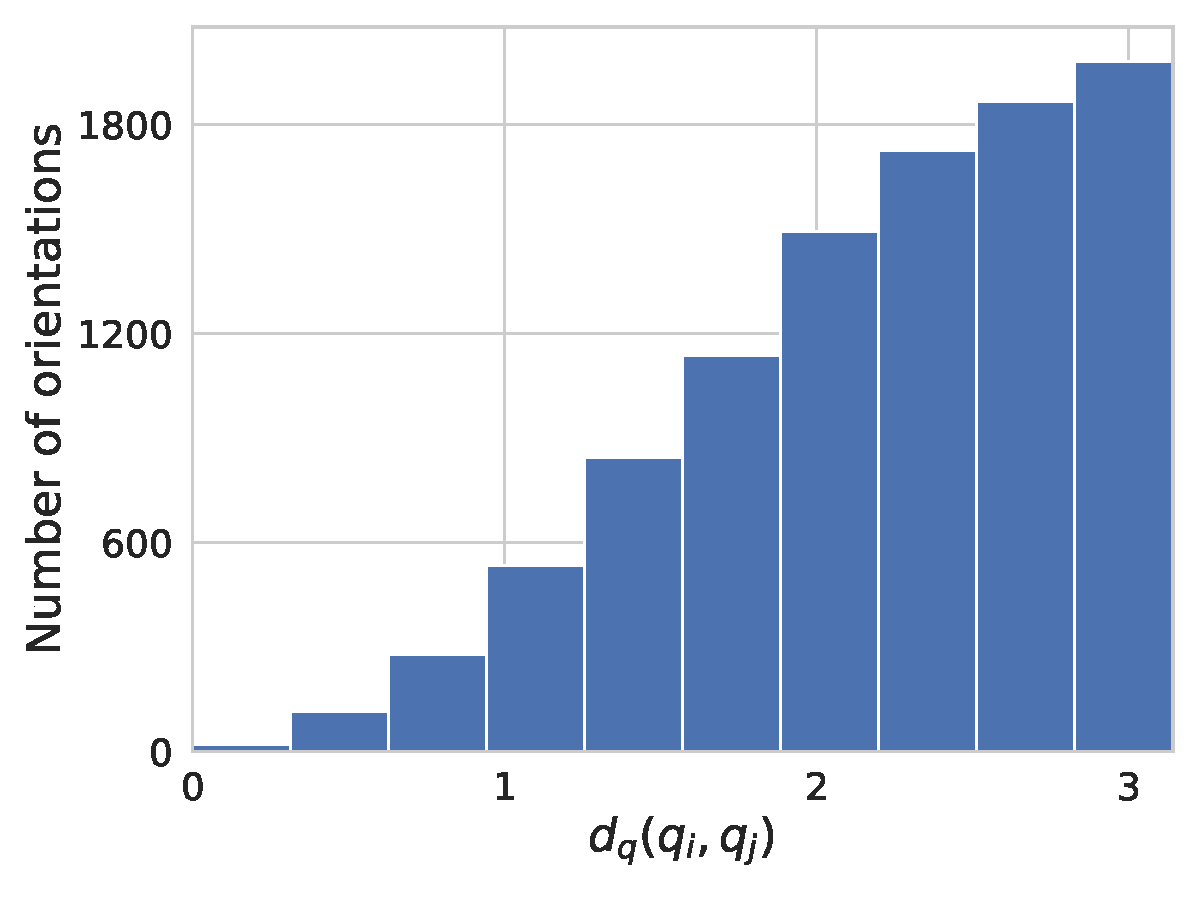
\includegraphics[height=8em]{figures/dQ_5j0n_uniform_quaternions.pdf}
        \caption{Distribution of ($10,000<P^2$) distances.}
    \end{subfigure}
    \hfill
    \begin{subfigure}[b]{0.62\linewidth}
        \centering
        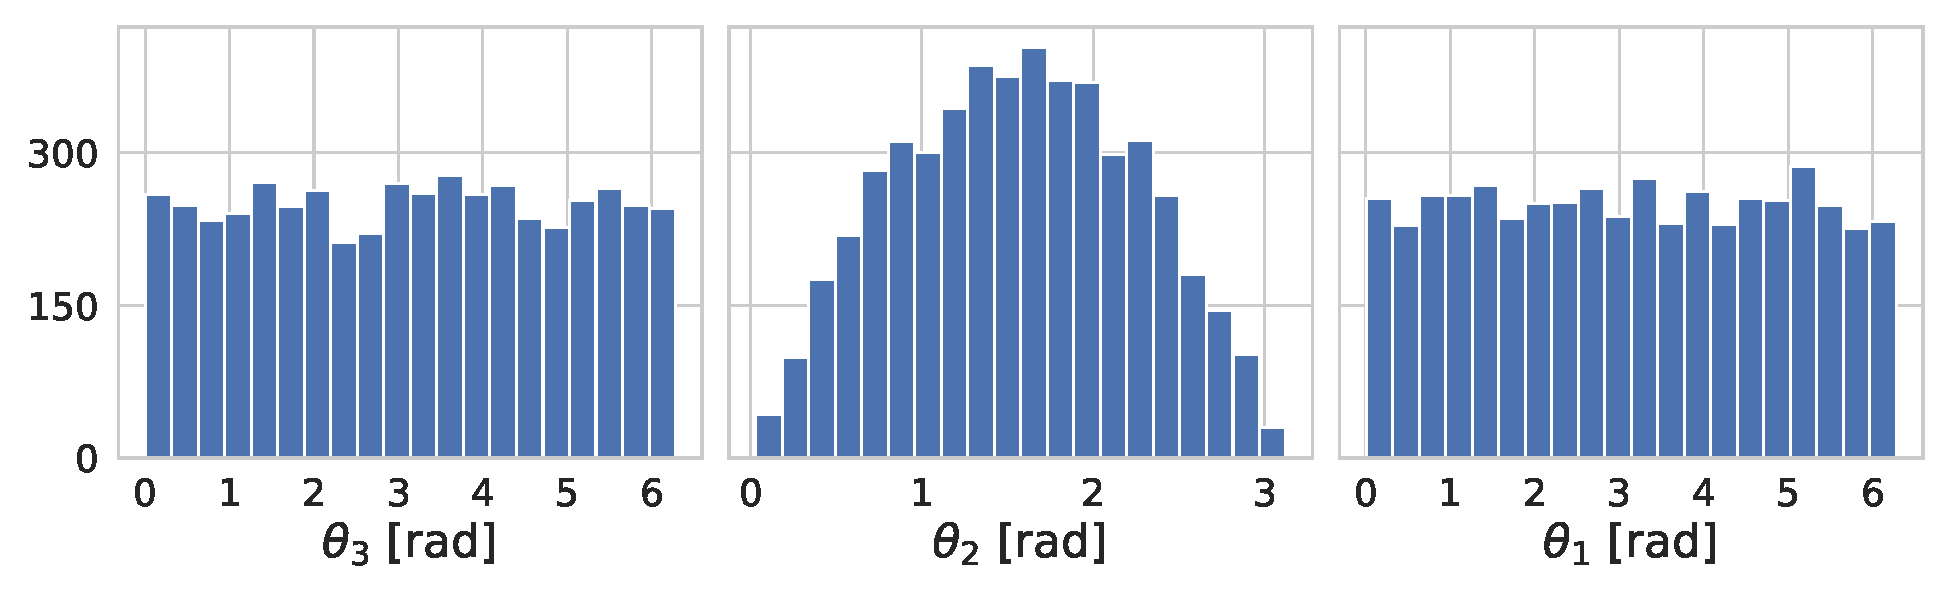
\includegraphics[height=8em]{figures/uniform_quaternions_ang.pdf}
        \caption{Distribution of Euler angles $\bth = (\theta_3,\theta_2,\theta_1)$.}
    \end{subfigure}
    \\ \vspace{1em}
    \begin{subfigure}[b]{0.36\linewidth}
        \centering
        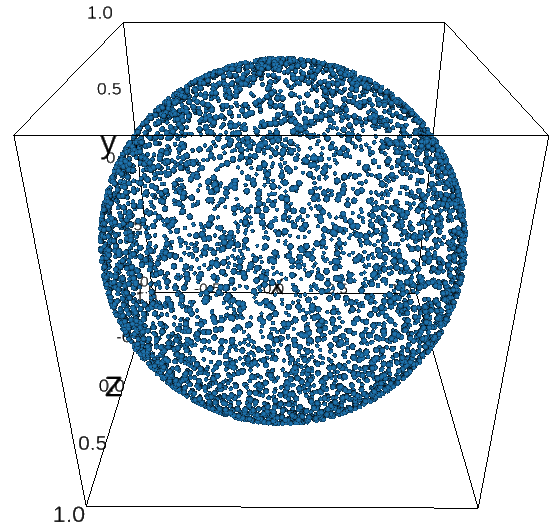
\includegraphics[height=8em]{figures/uniform_quaternion.png}
        \caption{Sampled directions $(\theta_2, \theta_1)$.}
    \end{subfigure}
    \hfill
    \begin{subfigure}[b]{0.62\linewidth}
        \centering
        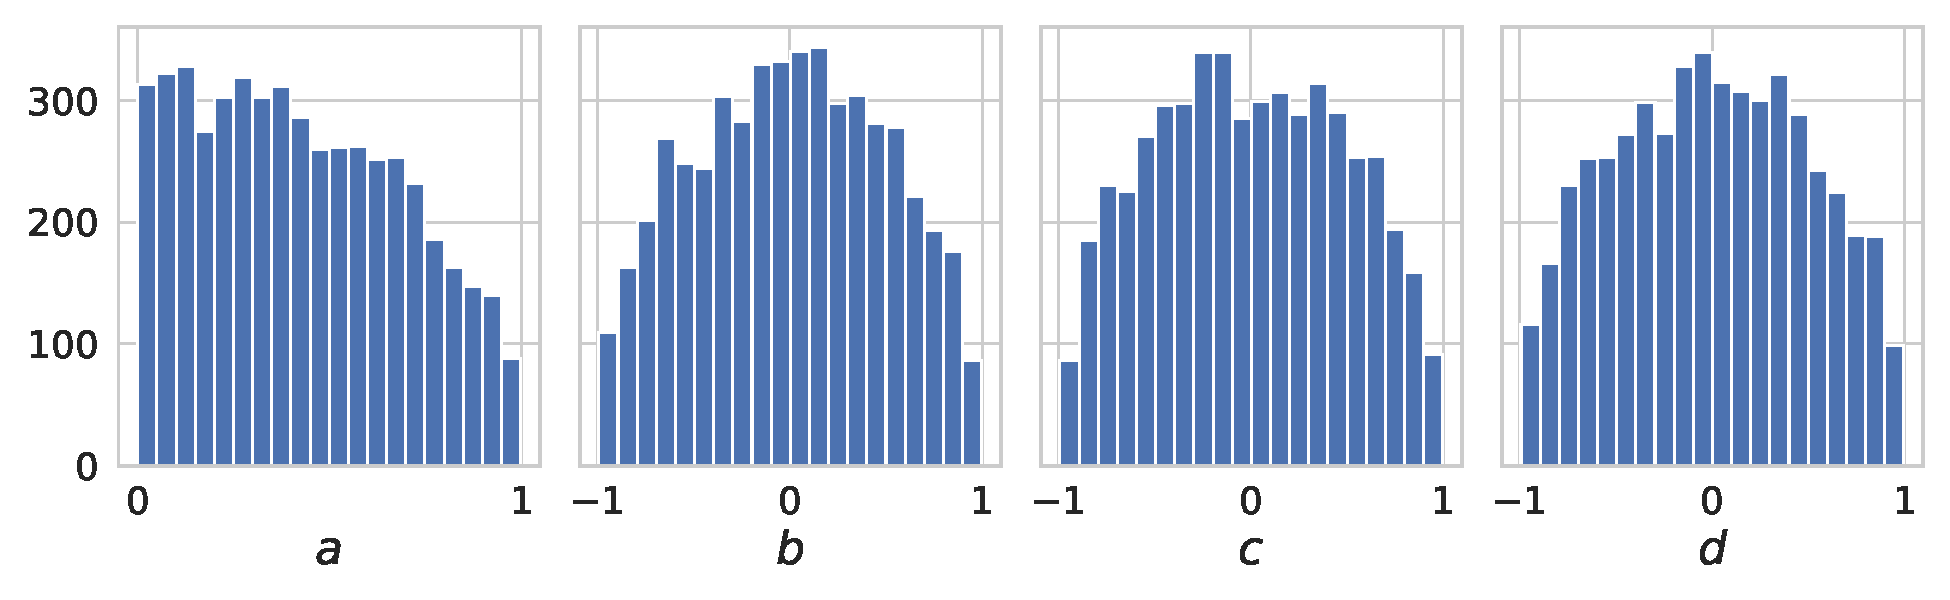
\includegraphics[height=8em]{figures/uniform_quaternions_q.pdf}
        \caption{Distribution of quaternions $q = a + b\boldsymbol{i} + c\boldsymbol{j} + d\boldsymbol{k}$.}
    \end{subfigure}
    \caption{%
        Uniform sampling of $P=5,000$ orientations from $\SO(3)$.
        %\mdeff{That's not uniform in quaternion space, as shown by (d). ;) It's uniform in rotation / SO(3) space. How did you sample it? A classic way is to draw from $\mathcal{N}(0, I_4)$ then normalize to unit norm. More at \url{https://mathworld.wolfram.com/SpherePointPicking.html}.}\banjac{yes, we sample uniformly on SO(3), sorry my mistake in wording}
        \mdeff{I'd like to merge \figref{uniform-orientations} and \figref{uniform-angles} (they take a lot of space). We could keep the two spheres (c), but merge the histograms (a,b,d) by using one color for $\SO(3)$ uniform and another color for Euler uniform (like in \figref{orientation-constraints}c).}
    }\label{fig:uniform-orientations}
\end{figure}

\begin{figure}[ht!]
    \centering
    \begin{subfigure}[b]{0.36\linewidth}
        \centering
        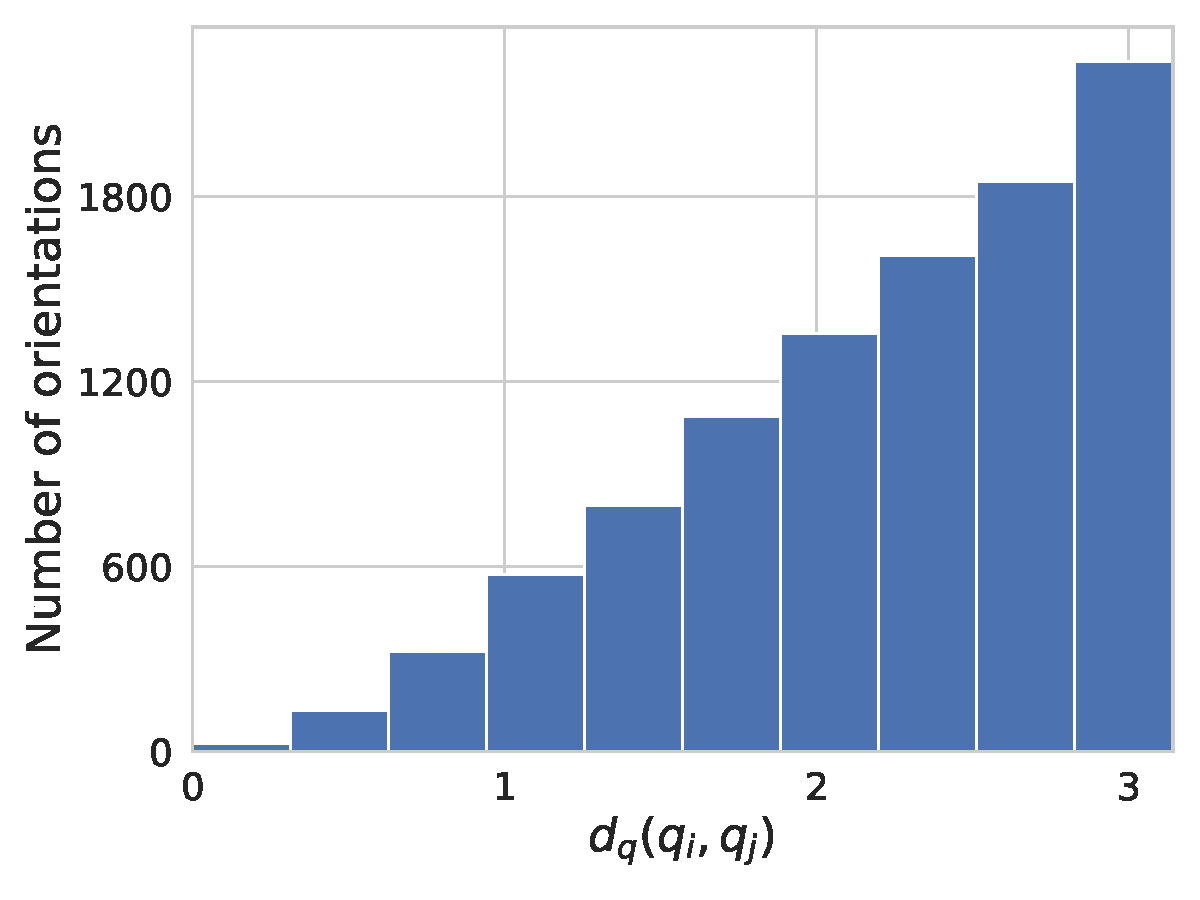
\includegraphics[height=8em]{figures/dQ_5j0n_uniform_angles.pdf}
        \caption{Distribution of ($10,000<P^2$) distances.}
    \end{subfigure}
    \hfill
    \begin{subfigure}[b]{0.62\linewidth}
        \centering
        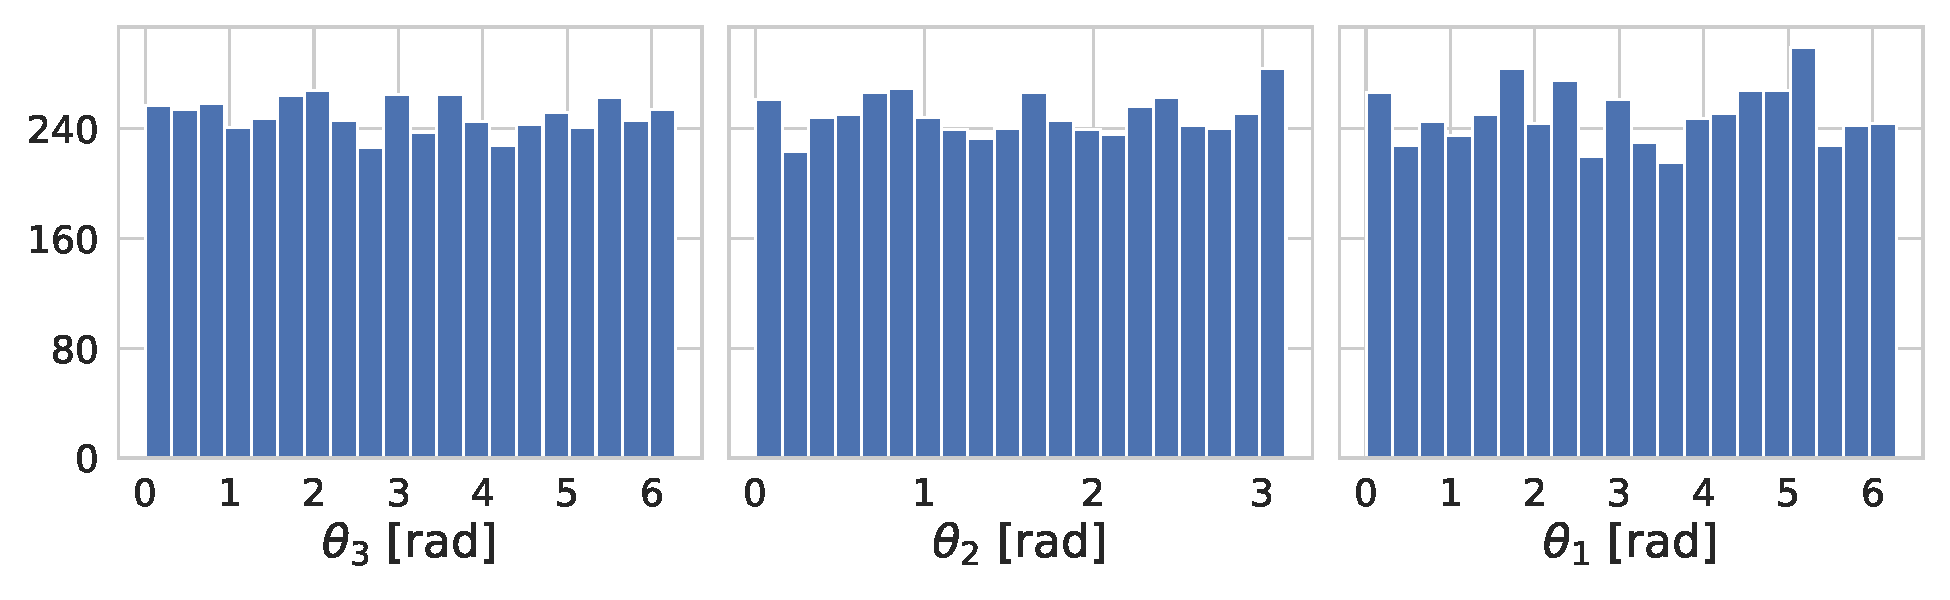
\includegraphics[height=8em]{figures/uniform_angles_ang.pdf}
        \caption{Distribution of Euler angles $\bth = (\theta_3,\theta_2,\theta_1)$.}
    \end{subfigure}
    \\ \vspace{1em}
    \begin{subfigure}[b]{0.36\linewidth}
        \centering
        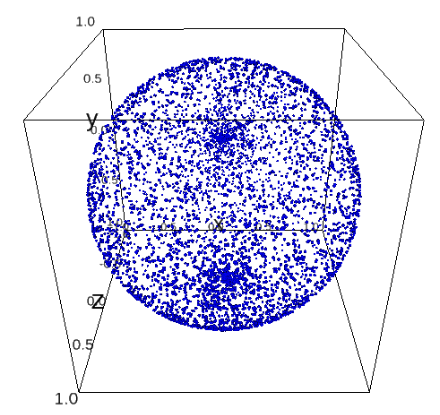
\includegraphics[height=8em]{figures/uniform_angles.png}
        \caption{Sampled directions $(\theta_2, \theta_1)$.}
    \end{subfigure}
    \hfill
    \begin{subfigure}[b]{0.62\linewidth}
        \centering
        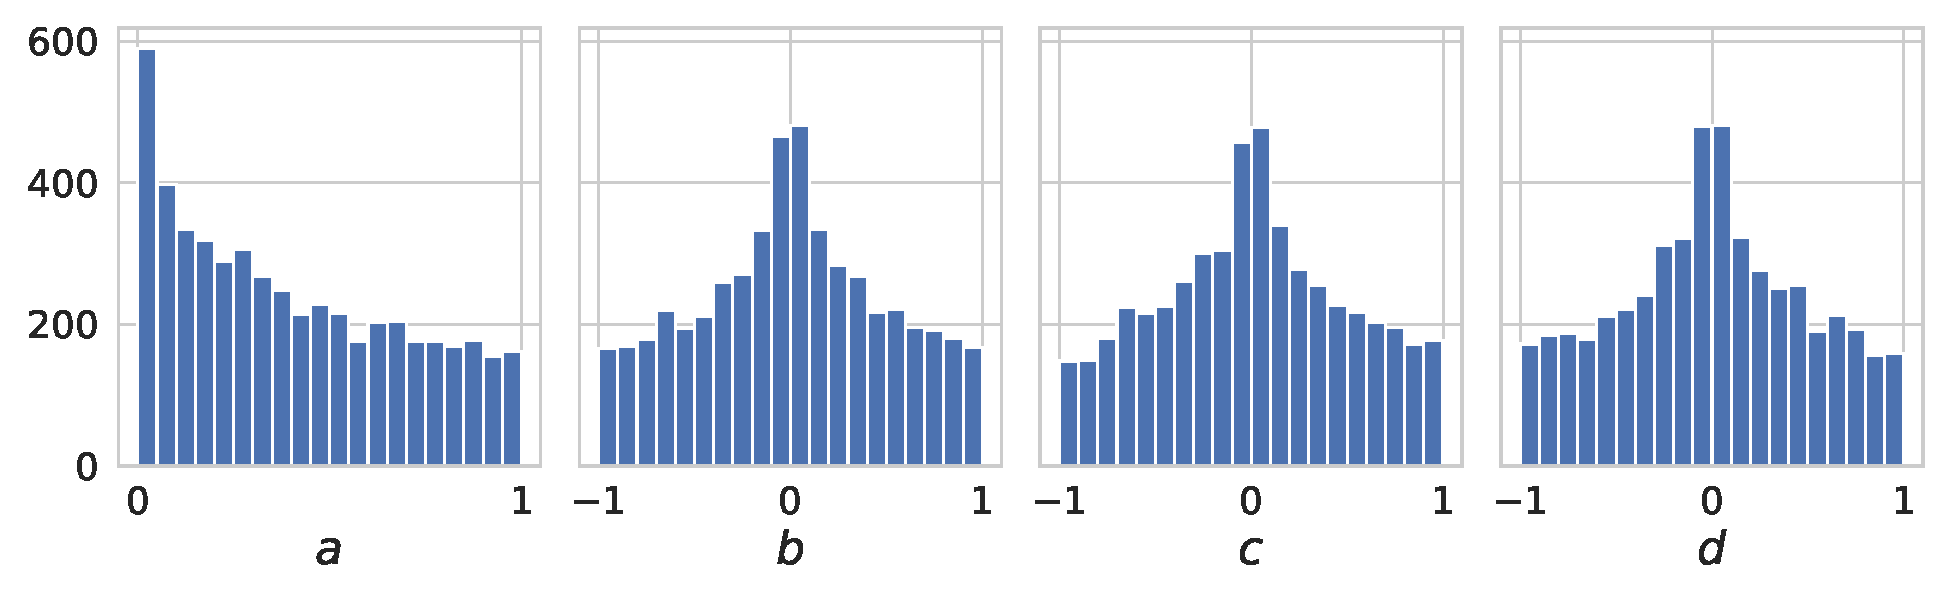
\includegraphics[height=8em]{figures/uniform_angles_q.pdf}
        \caption{Distribution of quaternions $q = a + b\boldsymbol{i} + c\boldsymbol{j} + d\boldsymbol{k}$.}
    \end{subfigure}
     \caption{%
        Uniform sampling of $P=5,000$ Euler angles from $[0,2\pi[ \, \times \, [0,\pi] \times [0,2\pi[$ inducing a non-uniform distribution of orientations.
    }\label{fig:uniform-angles}
\end{figure}

\figref{orientation-constraints} shows distributions of induced distances when directions $(\theta_2, \theta_1)$ are constrained to an half or a quarter of the 2-sphere.
% (to learn from asymmetric proteins like \texttt{5j0n})
% (\eg, for proteins with D2 symmetry like \texttt{5a1a})
While the distributions flatten (compare with Figures~\ref{fig:uniform-orientations},\ref{fig:uniform-angles}a), the shorter distances are still way under-sampled.

\begin{figure}[ht!]
    \centering
    \begin{subfigure}[t]{0.32\linewidth}
        \centering
        %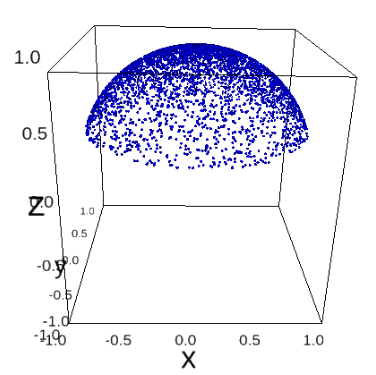
\includegraphics[height=7em]{figures/5j0n-half.png}
        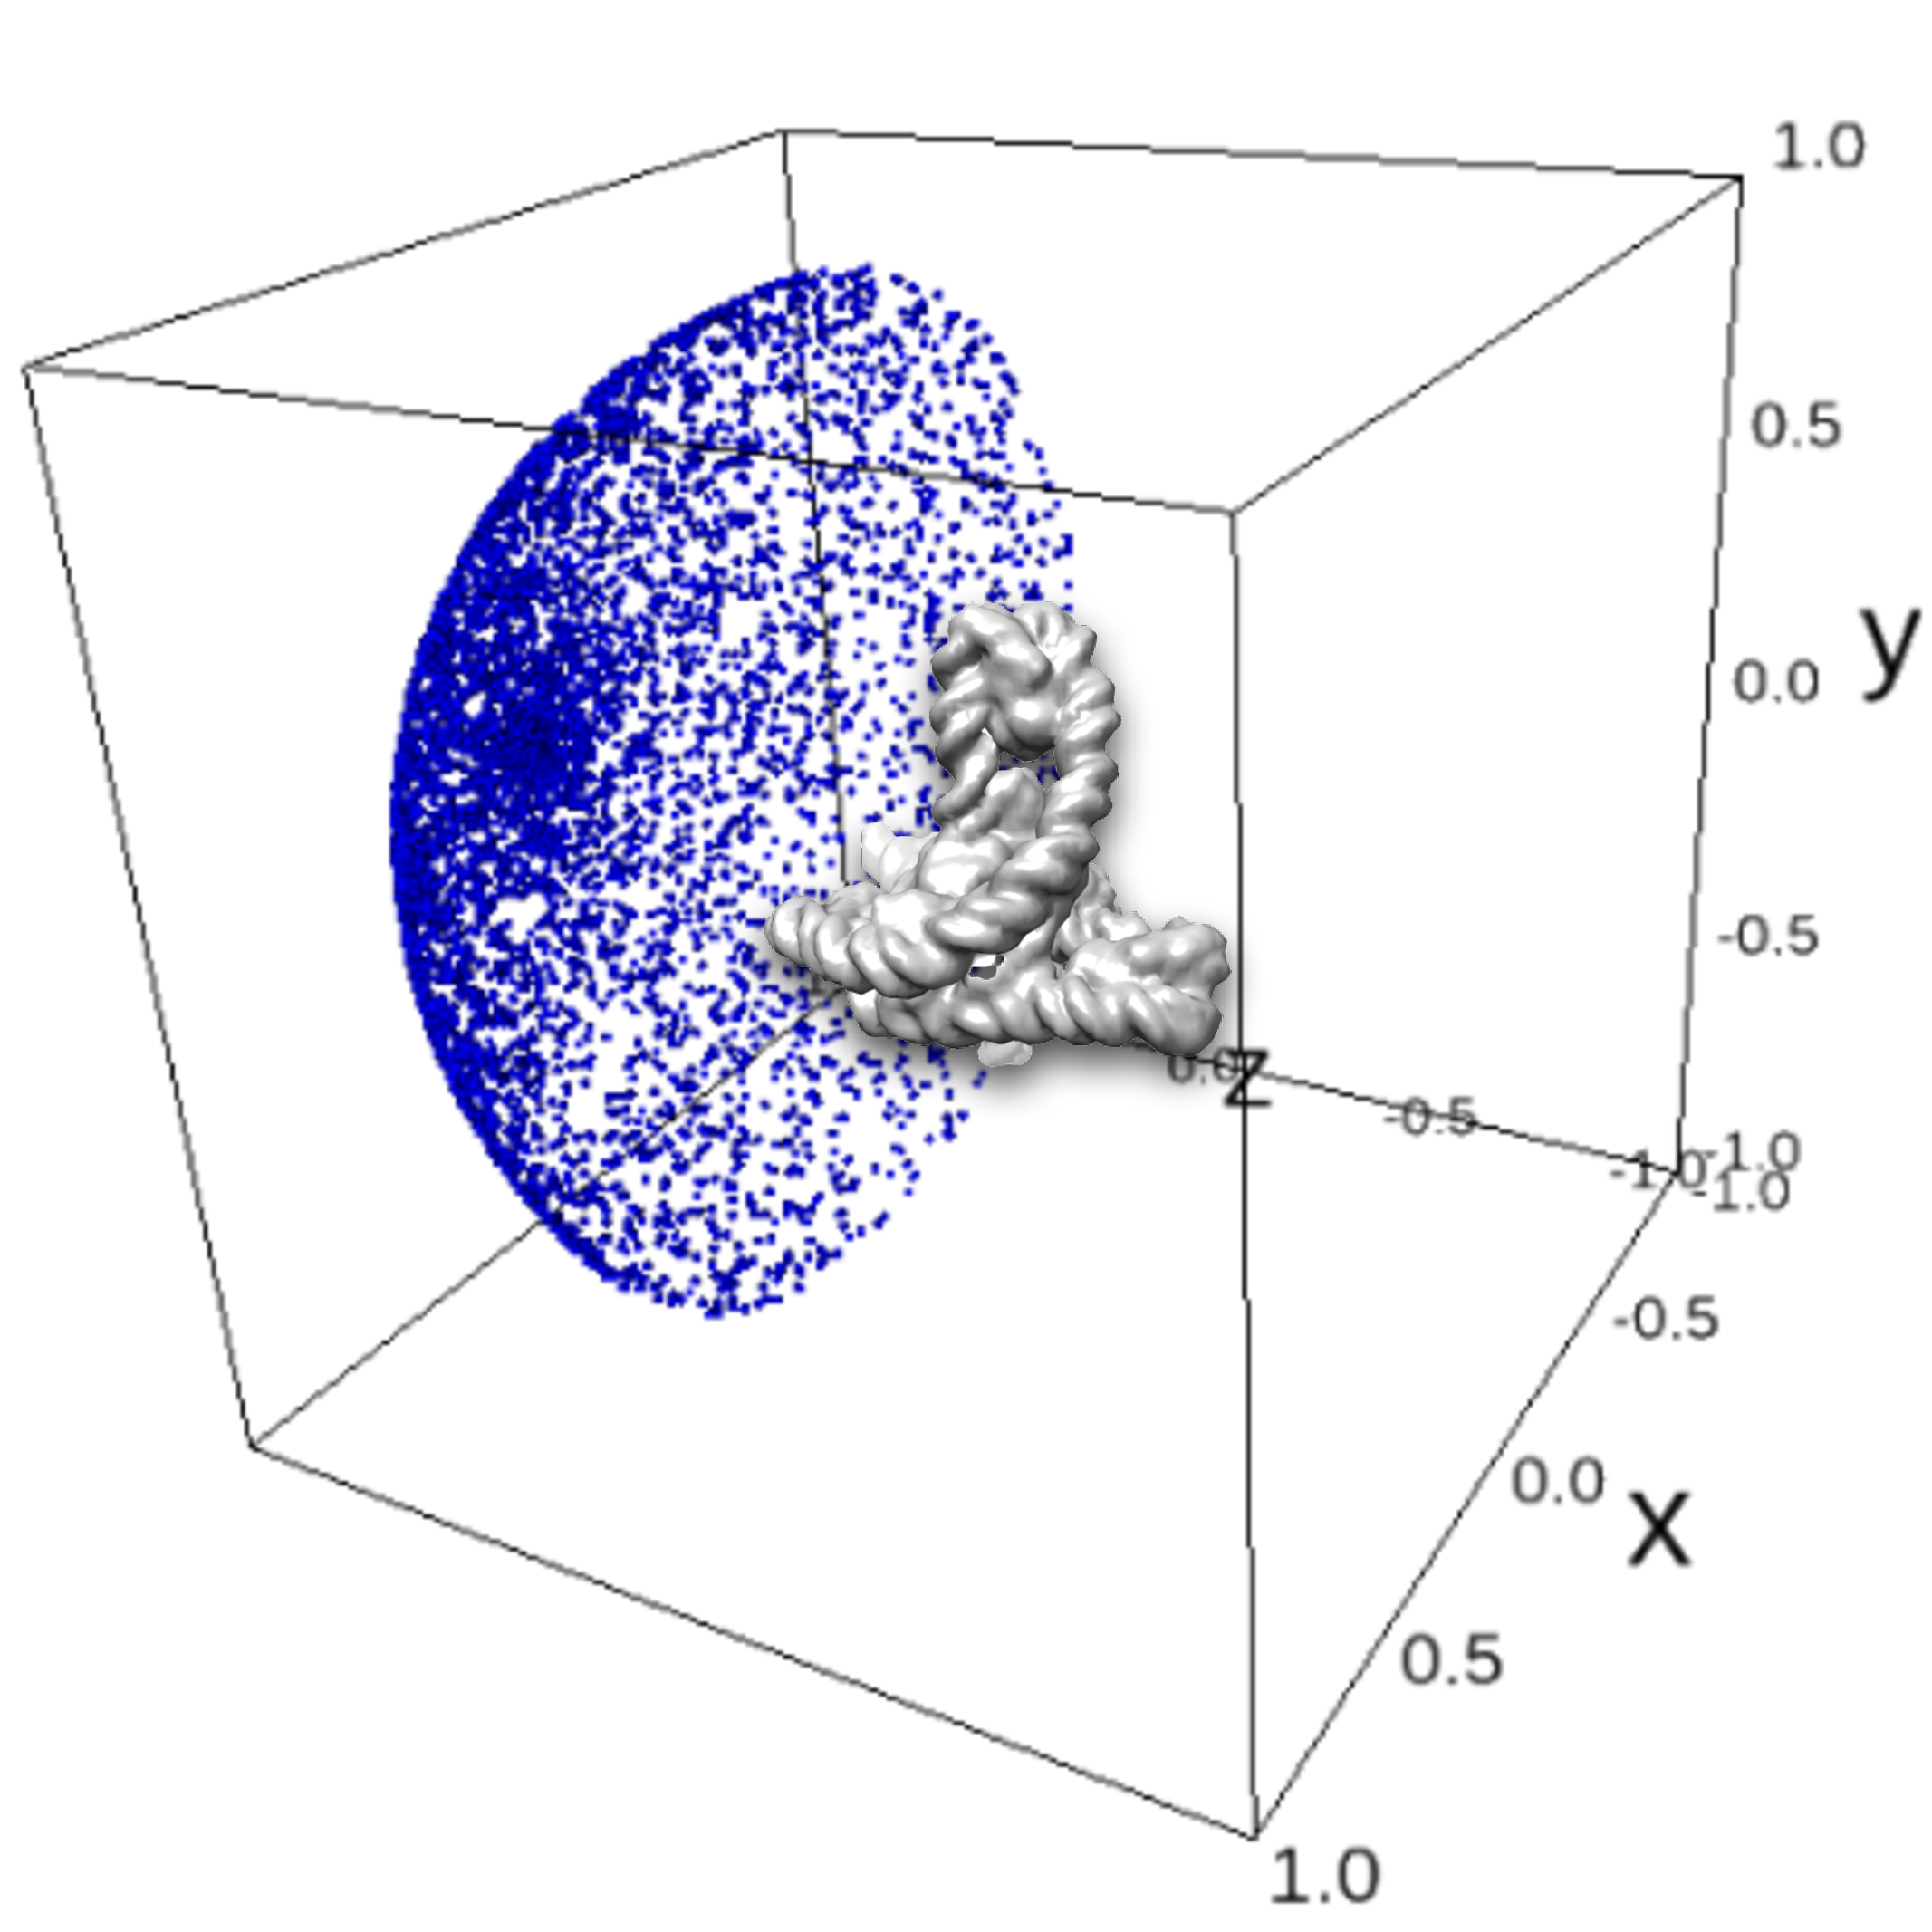
\includegraphics[height=9em]{figures/5j0n-cvg.pdf}
        \caption{Directions sampled from $(\theta_2, \theta_1) \in [0,\frac{\pi}{2}[ \, \times \, [0,2\pi[$, an half of the 2-sphere.}
    \end{subfigure}
    \hfill
    \begin{subfigure}[t]{0.32\linewidth}
        \centering
        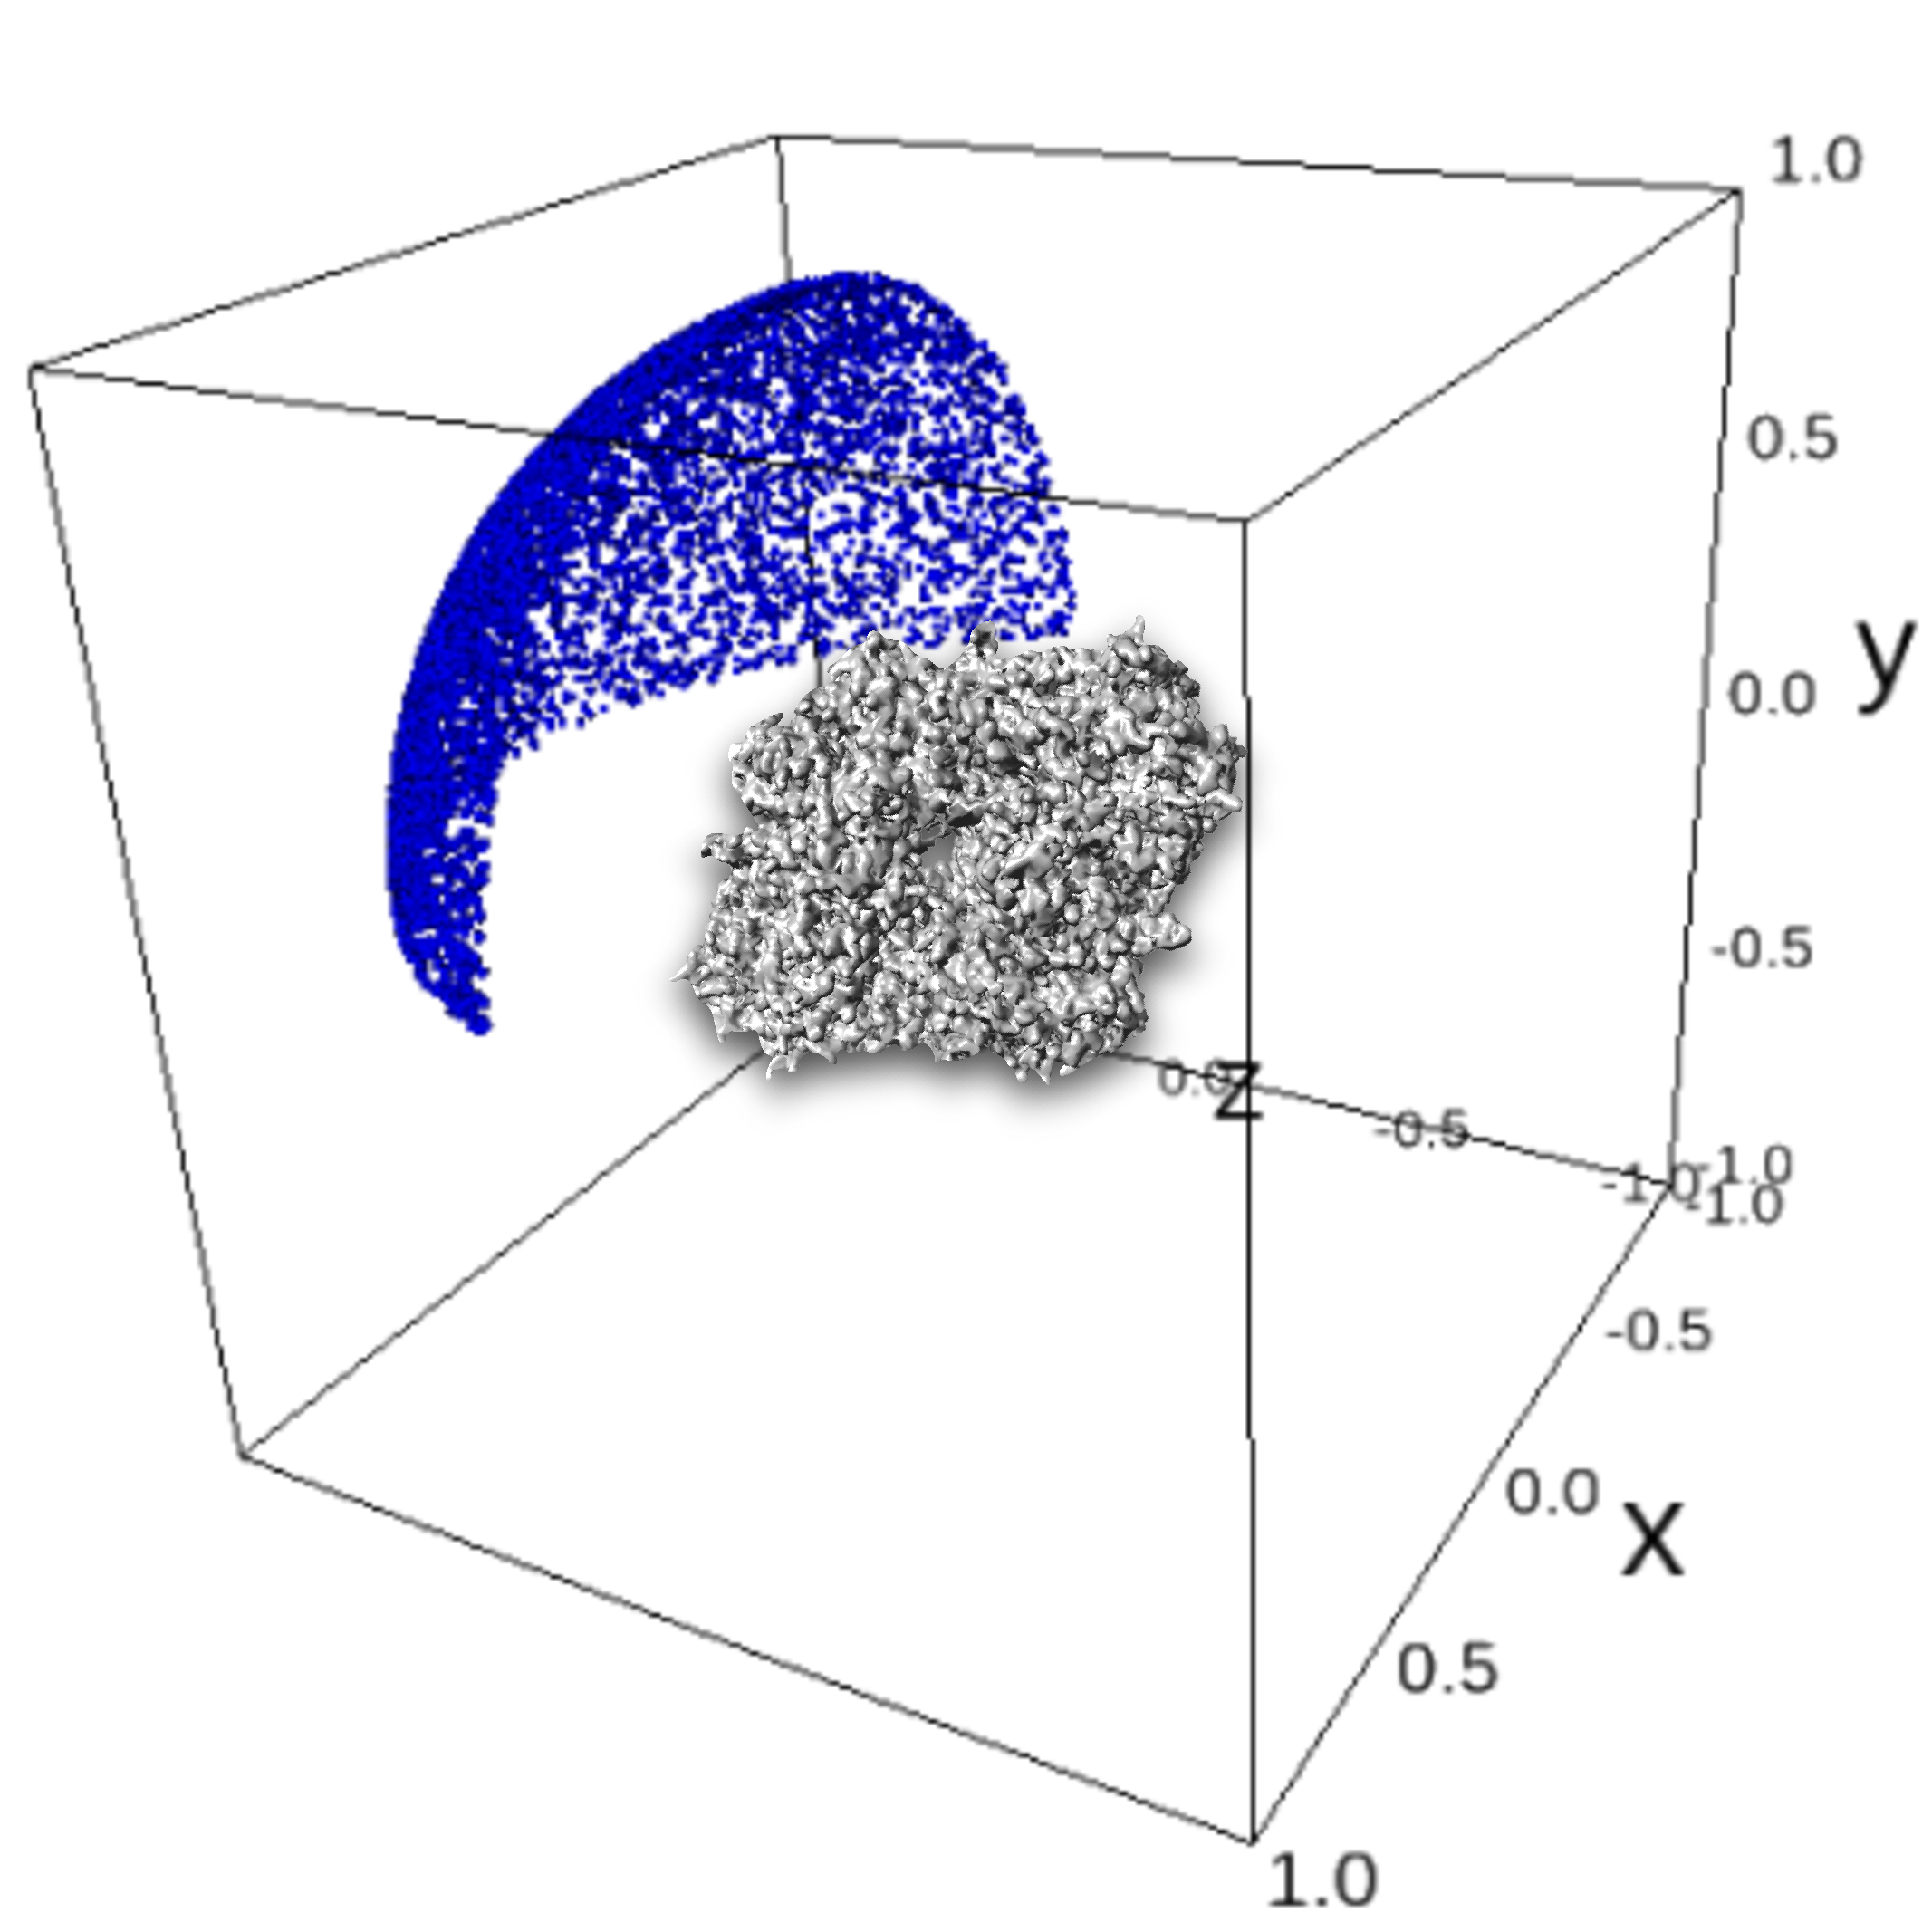
\includegraphics[height=9em]{figures/5a1a-cvg.pdf}
        \caption{Directions sampled from $(\theta_2, \theta_1) \in [0,\frac{\pi}{2}[ \, \times \, [0,\pi[$, a quarter of the 2-sphere.}
    \end{subfigure}
    \hfill
    \begin{subfigure}[t]{0.32\linewidth}
        \centering
        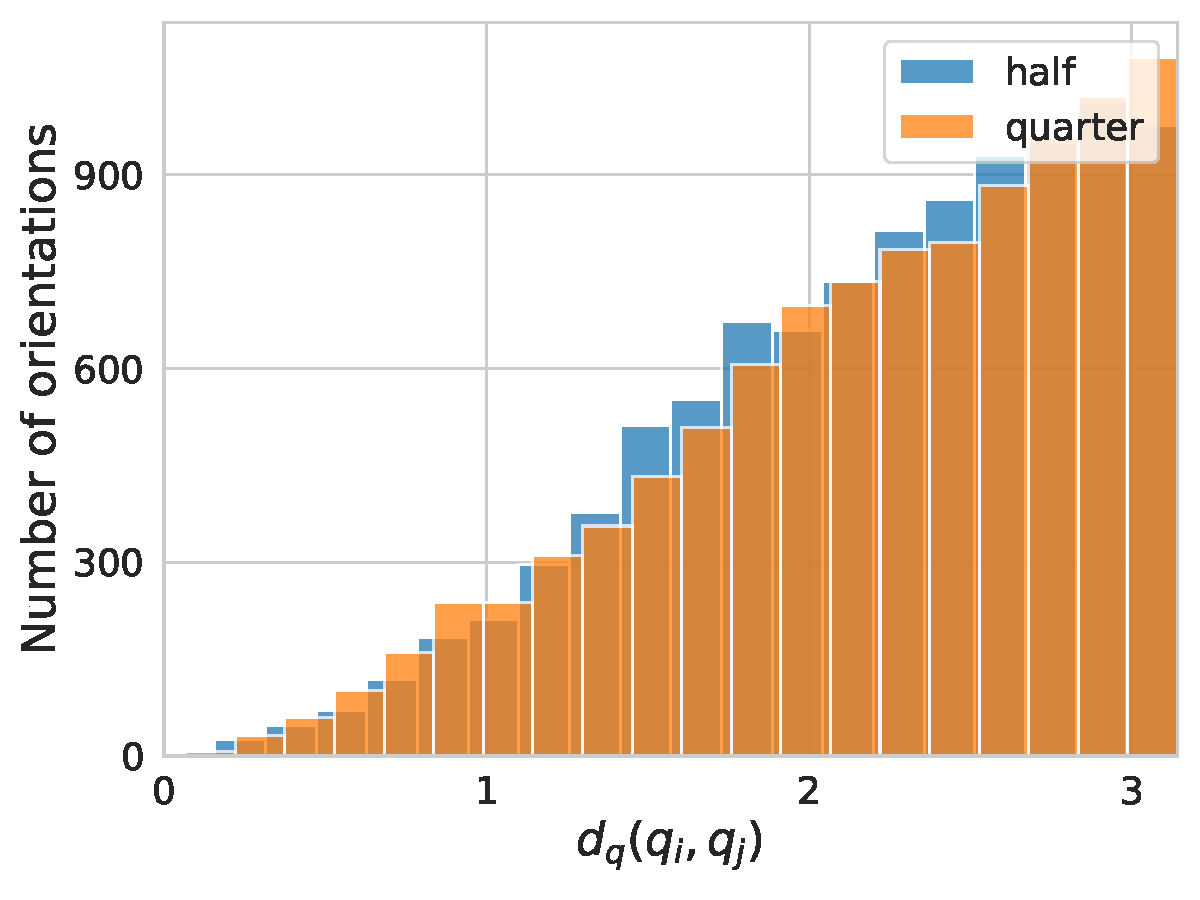
\includegraphics[height=9em]{figures/dQ_half_vs_quarter.pdf}
        \caption{Induced distribution of distances.}
    \end{subfigure}
    \caption{%
        Distributions of $P=5,000$ directions $(\theta_2, \theta_1)$ as points on the 2-sphere (see also \figref{imaging-geometry}), illustrating their constrained range, and the distances they induce.
    }\label{fig:orientation-constraints}
\end{figure}

\begin{figure}[ht!]
    \centering
    \begin{subfigure}[b]{0.55\linewidth}
        \centering
        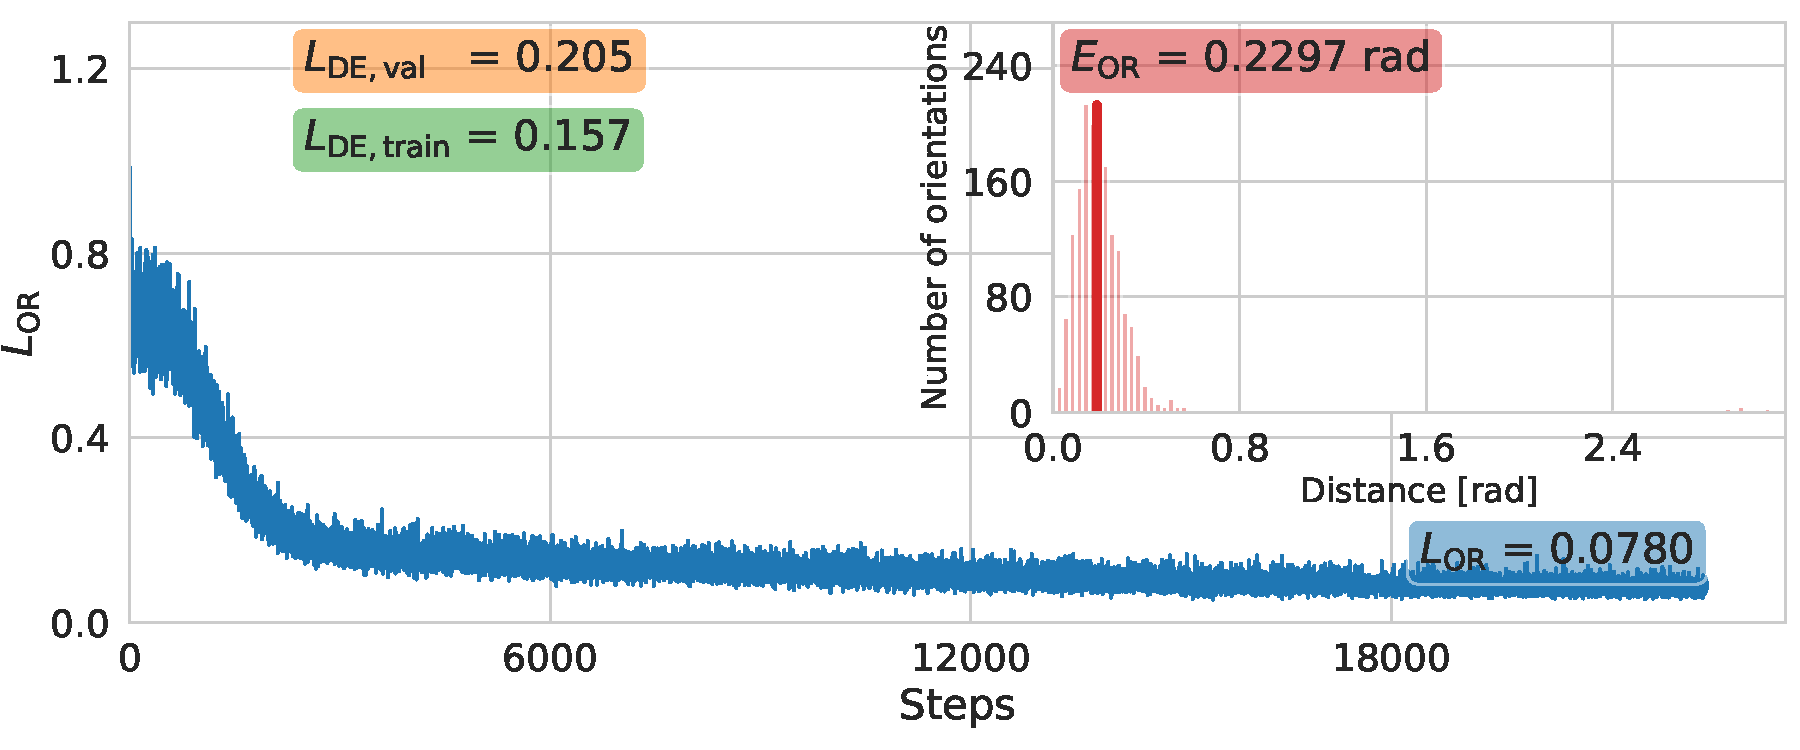
\includegraphics[height=11em]{figures/5j0n_ar_aa_fullcvg.pdf}
        \caption{Recovered $\{ \widehat{q_i} \}$ from noiseless \texttt{5j0n} projections $\{ \p_i \}$.}
    \end{subfigure}
    \hfill
    \begin{subfigure}[b]{0.4\linewidth}
        \centering
        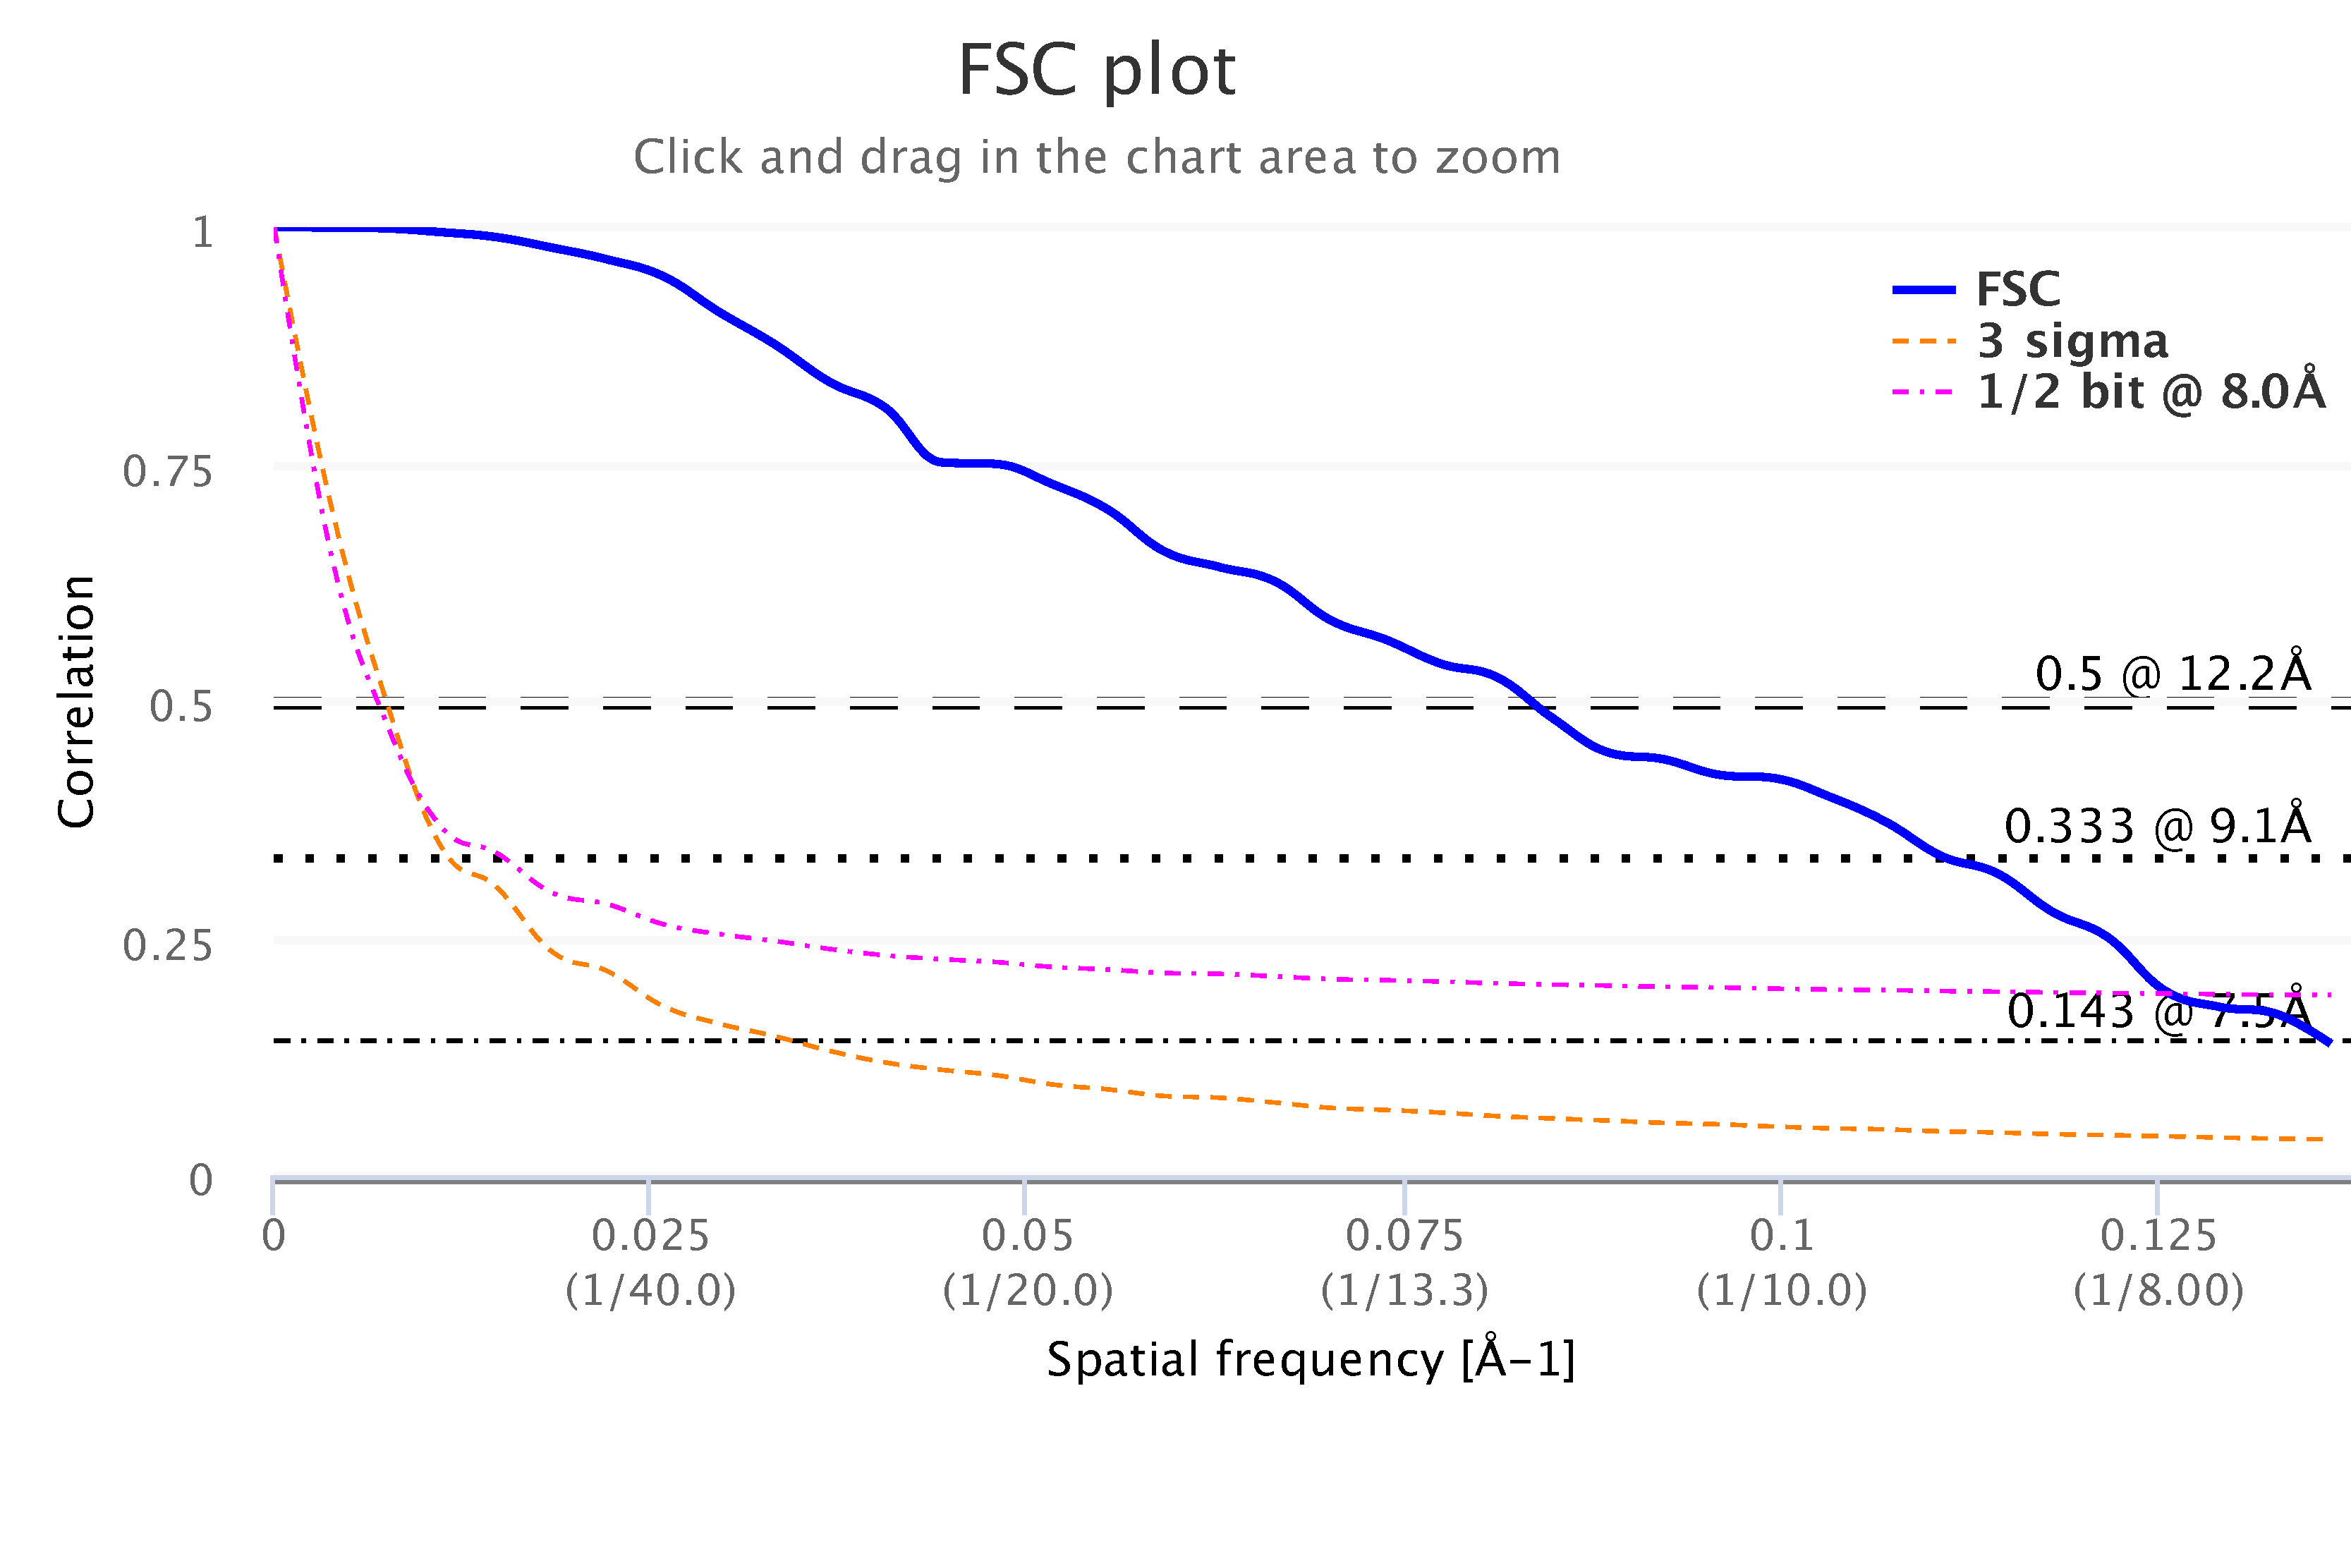
\includegraphics[height=11em]{figures/FSC_5j0n_fullcvg_noise0_fin_vs_init.pdf}
        \caption{Fourier Shell Correlation (FSC) of the reconstruction.}
    \end{subfigure}
    \caption{%
        Orientation recovery and density reconstruction from projections acquired from non-uniformly orientations (uniformly sampled Euler angles).
        %Full pipeline on the orientations with uniform sampling of Euler angles from full 2-sphere coverage.
    }\label{fig:recovery-nonuniform}
\end{figure}

\section{Orientation recovery from exact distances}\label{apx:results:orientation-recovery:exact}

%\mdeff{Story: works perfectly despite no convexity guarantee and sampling.}

\lau{Smooth.}
To verify that the lack of a convexity guarantee for \eqnref{orientation-recovery} and the sampling of the sum are non-issues in practice, we attempted orientation recovery under exact distance estimation $d_p(\p_i, \p_j) = d_q(q_i, q_j)$.
Orientations were perfectly recovered.
\figref{5j0n-orientation-recovery-loss} shows the convergence of the loss $L_\text{OR}$ to zero.
\figref{5j0n-aa-loss-perfect-distances} shows how~\eqnref{orientation-recovery-error} could then perfectly align the recovered and true orientations---leading to $E_\text{OR} = 0$.
% Demonstrating that alignment is necessary to evaluate the performance of orientation recovery.

\begin{figure}[ht!]
    \begin{minipage}[t]{0.37\linewidth}
        \centering
        %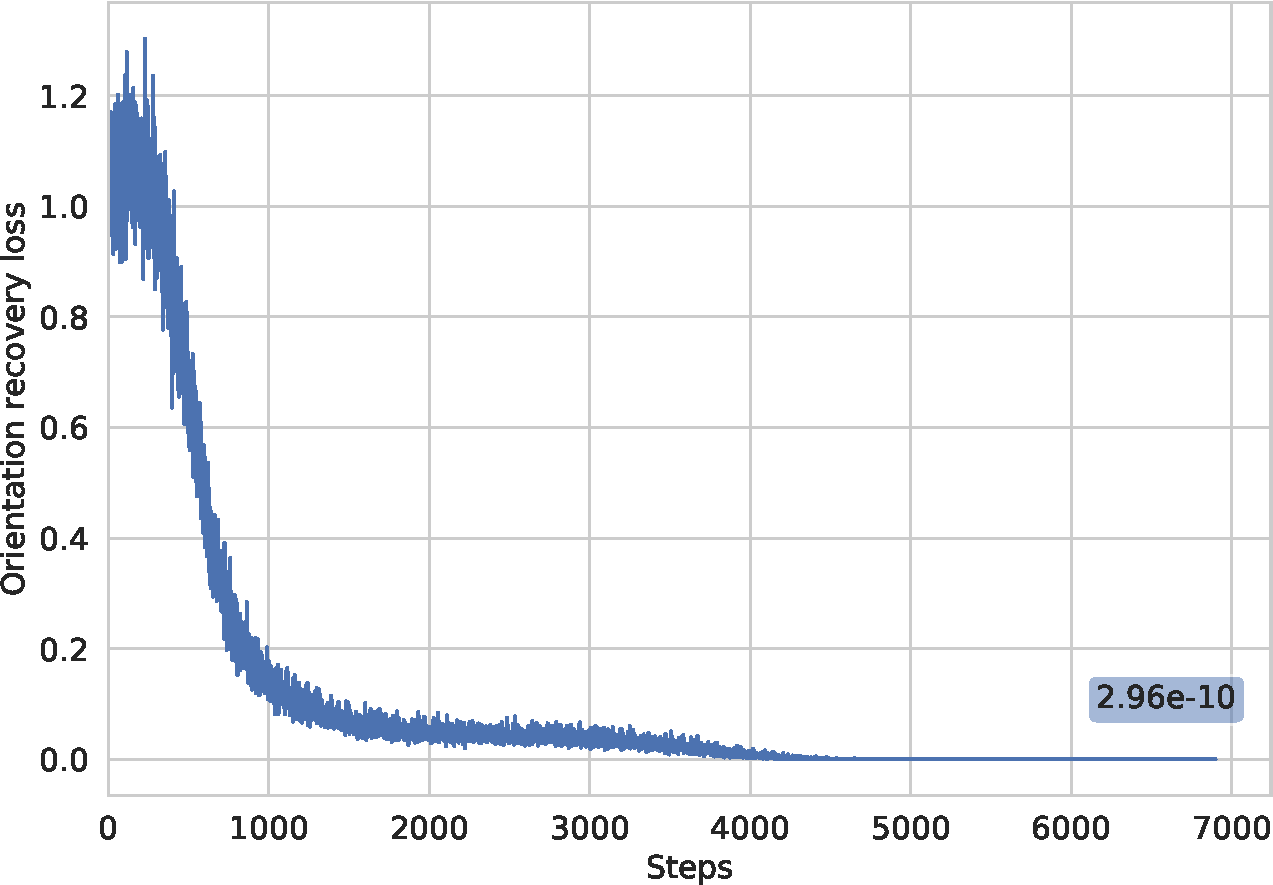
\includegraphics[height=3cm]{figures/5j0n_perfect_angle_recovery}
        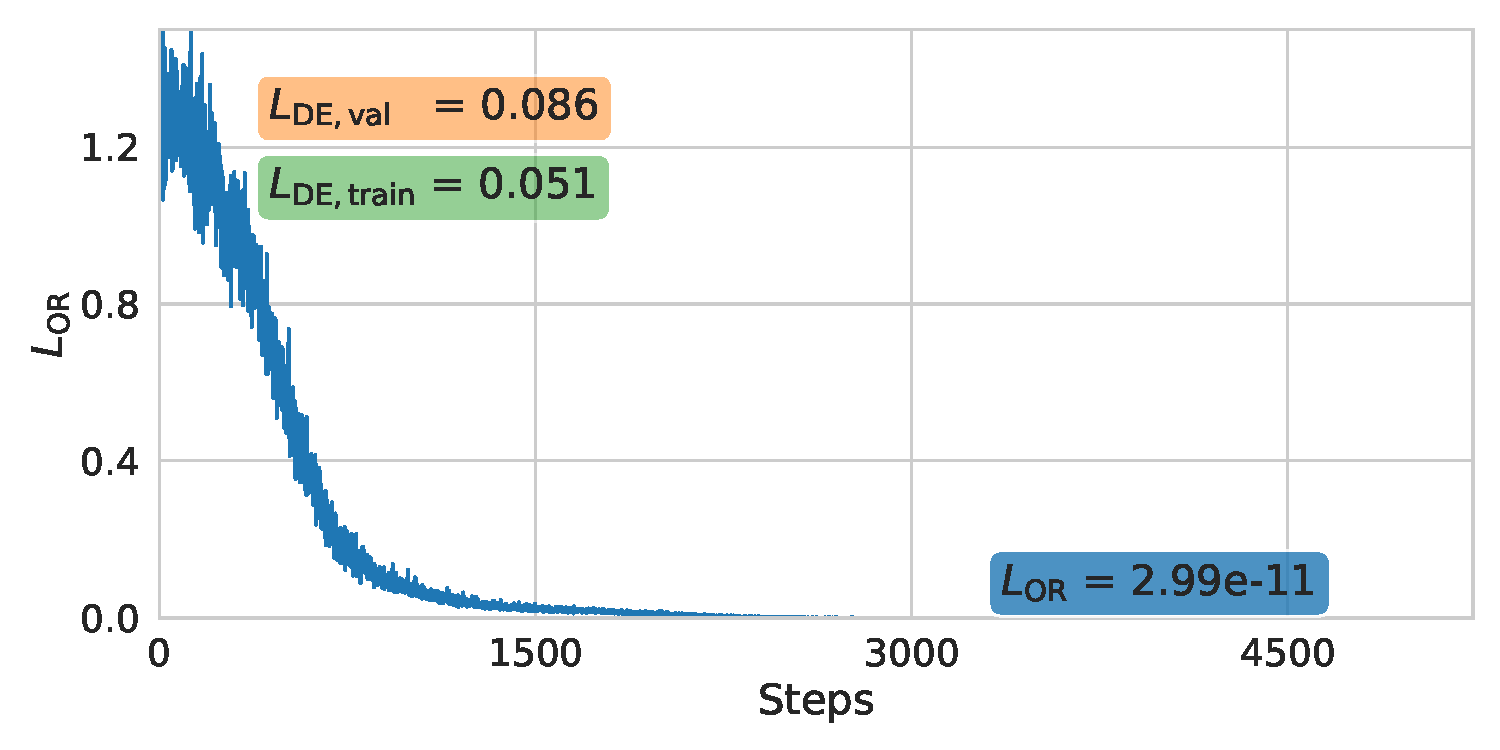
\includegraphics[height=3cm]{figures/5a1a_quartercov_uniformS2_halfInplane_ar_aa}
        \caption{%
            Example of perfect orientation recovery (for \texttt{5a1a}).
            The loss $L_\text{OR}$ \eqnref{orientation-recovery} converges to zero when the distance estimation is perfect, \ie, $\widehat{d_p}(\p_i, \p_j) = d_q(q_i, q_j)$.
        }\label{fig:5j0n-orientation-recovery-loss}
    \end{minipage}
    \hfill
    \begin{minipage}[t]{0.60\linewidth}
%        \begin{subfigure}[b]{0.19\linewidth}
%            \centering
%            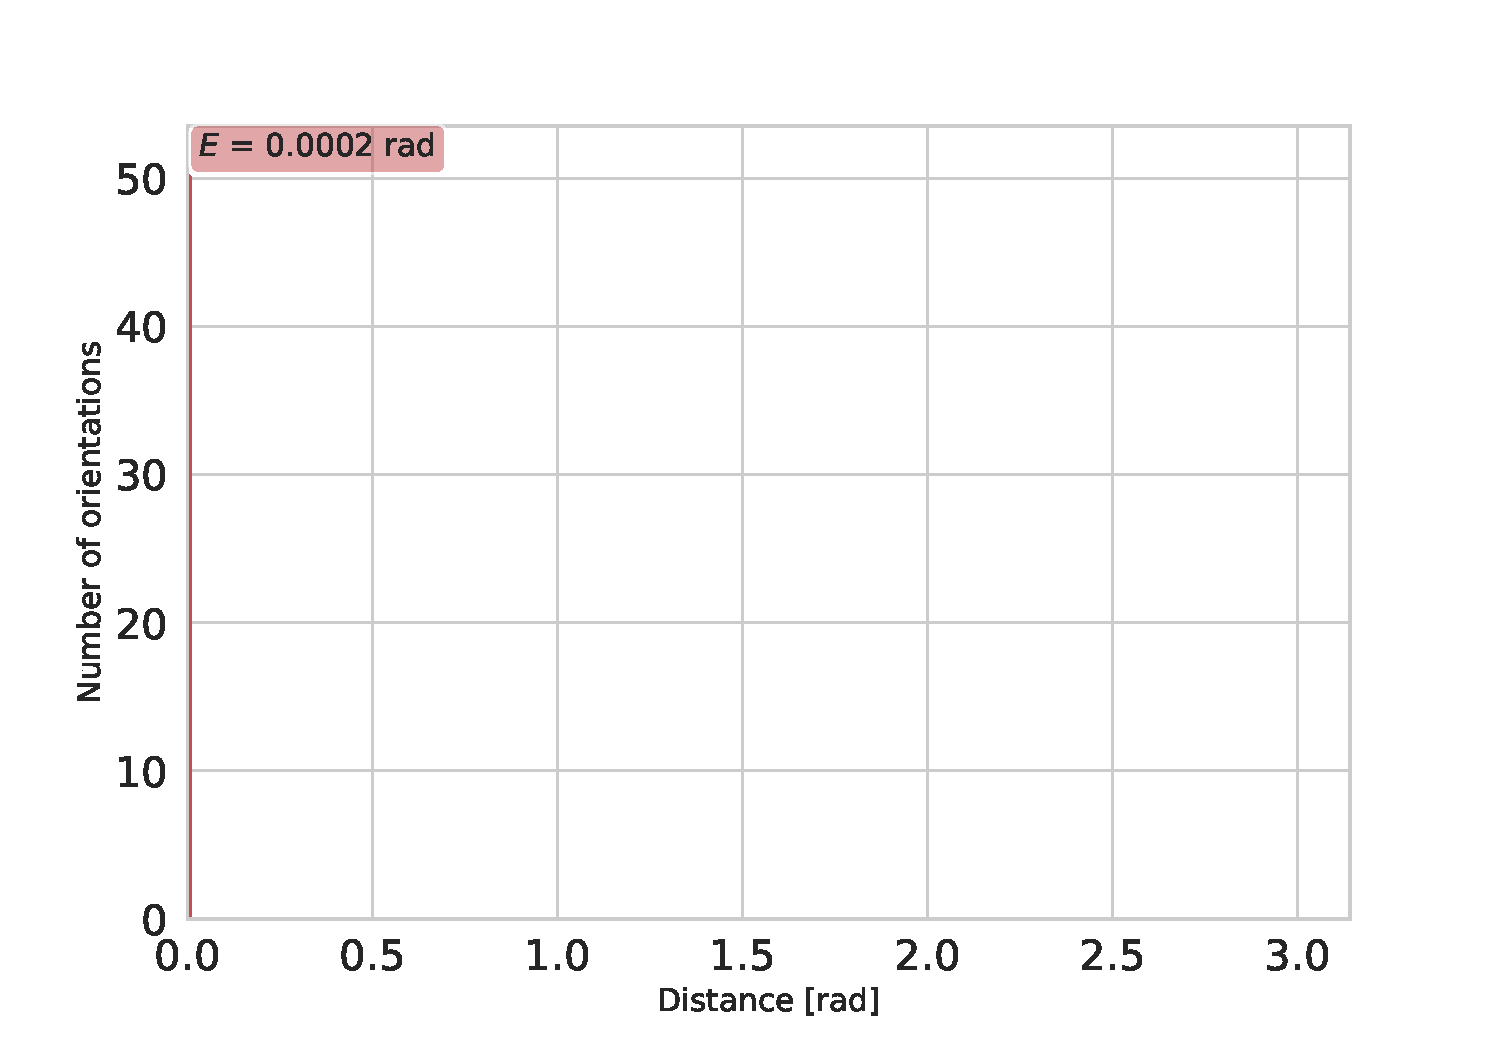
\includegraphics[height=3cm]{figures/5j0n_perfect_angle_ralignment_after}
%            \caption{Orientation recovery error with alignment.}
%        \end{subfigure}
%        \hfill
        % \begin{subfigure}[t]{4.3cm}
        %     \centering
        %     %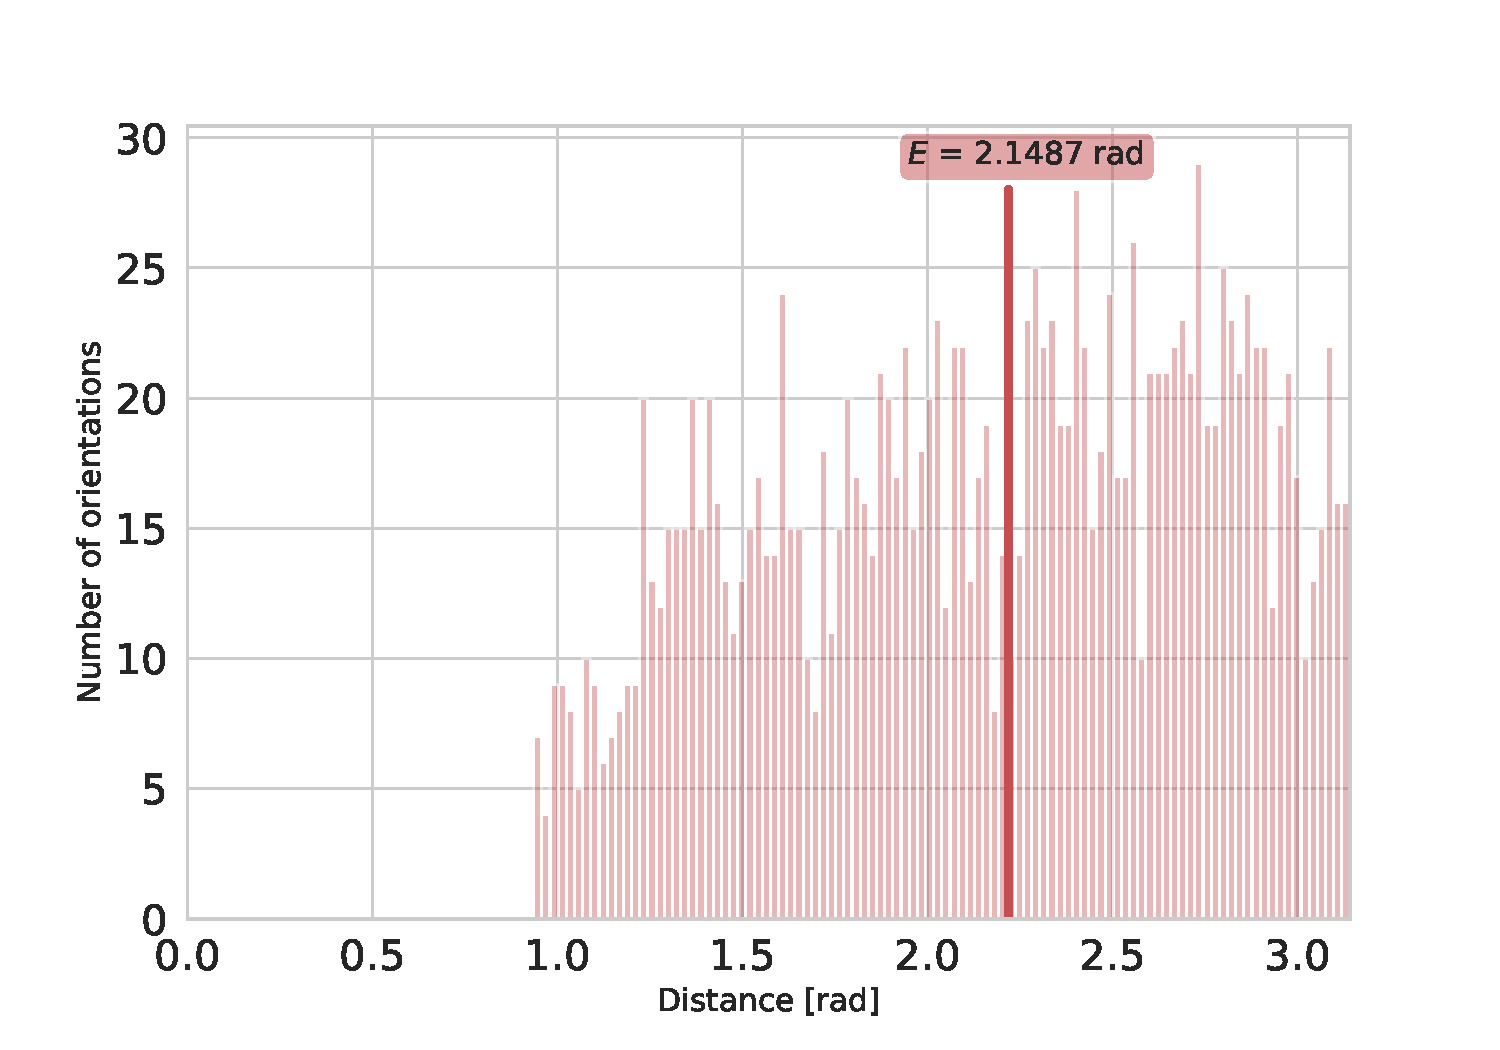
\includegraphics[height=3cm]{figures/5j0n_perfect_angle_ralignment_before}
        %     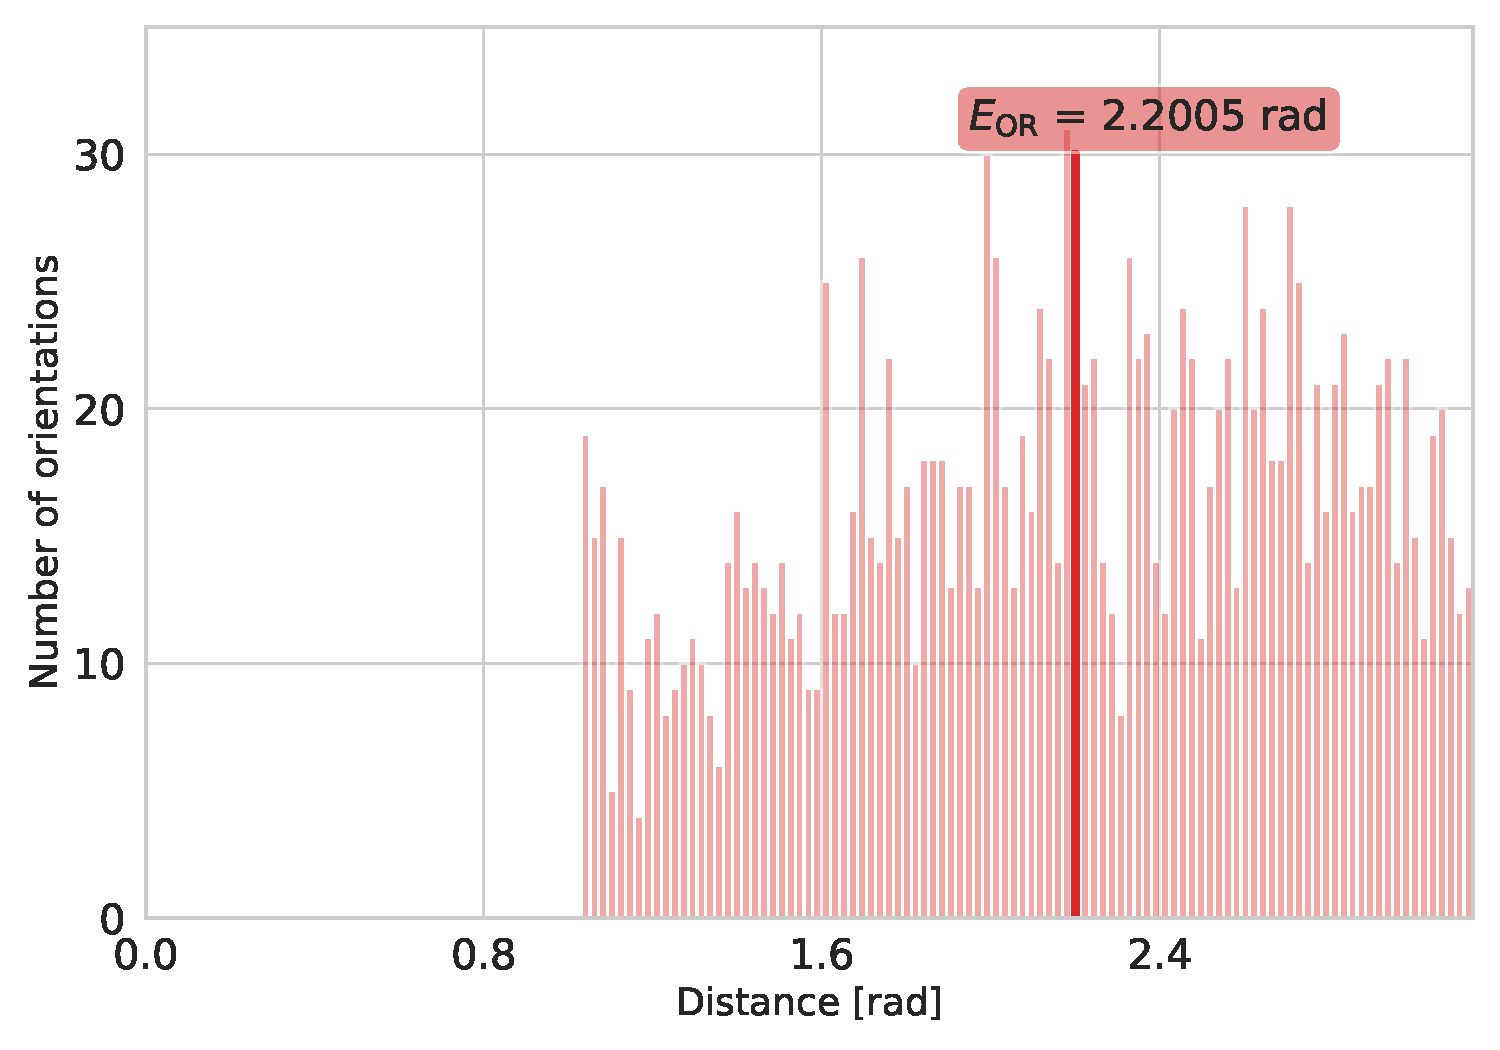
\includegraphics[height=3cm]{figures/5a1a_quartercov_uniformS2_halfInplane_before_alignment}
        %     \caption{Error histogram $\{ d_q (q_i, \widehat{q_i}) \}$, \ie, before alignment.}
        % \end{subfigure}
        % \hfill
        \begin{subfigure}[t]{0.46\linewidth}
            \centering
            % 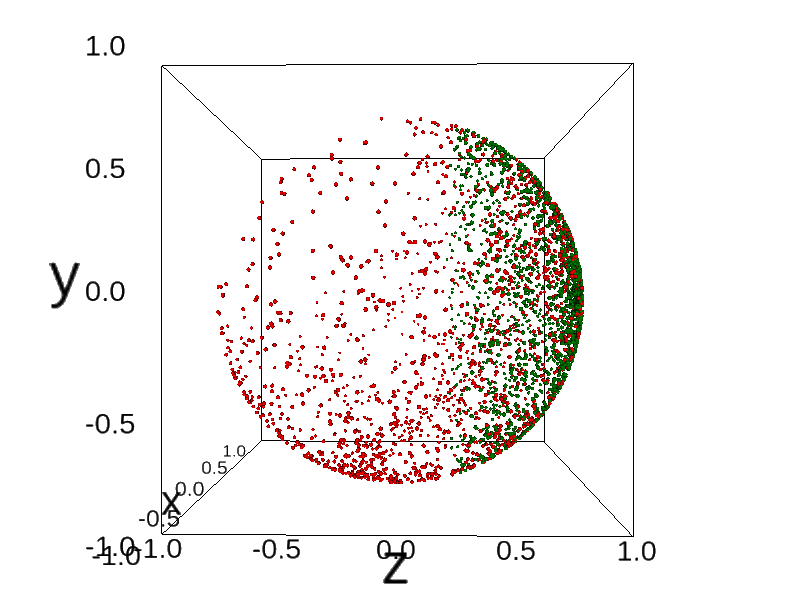
\includegraphics[height=3cm]{figures/coverage_alignment_before.png}
            %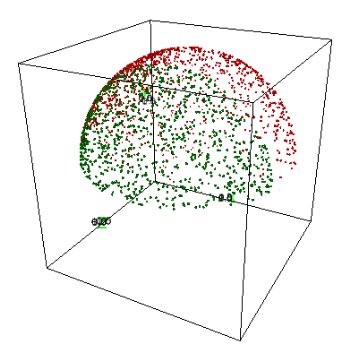
\includegraphics[height=3cm]{figures/before_aa.png}
            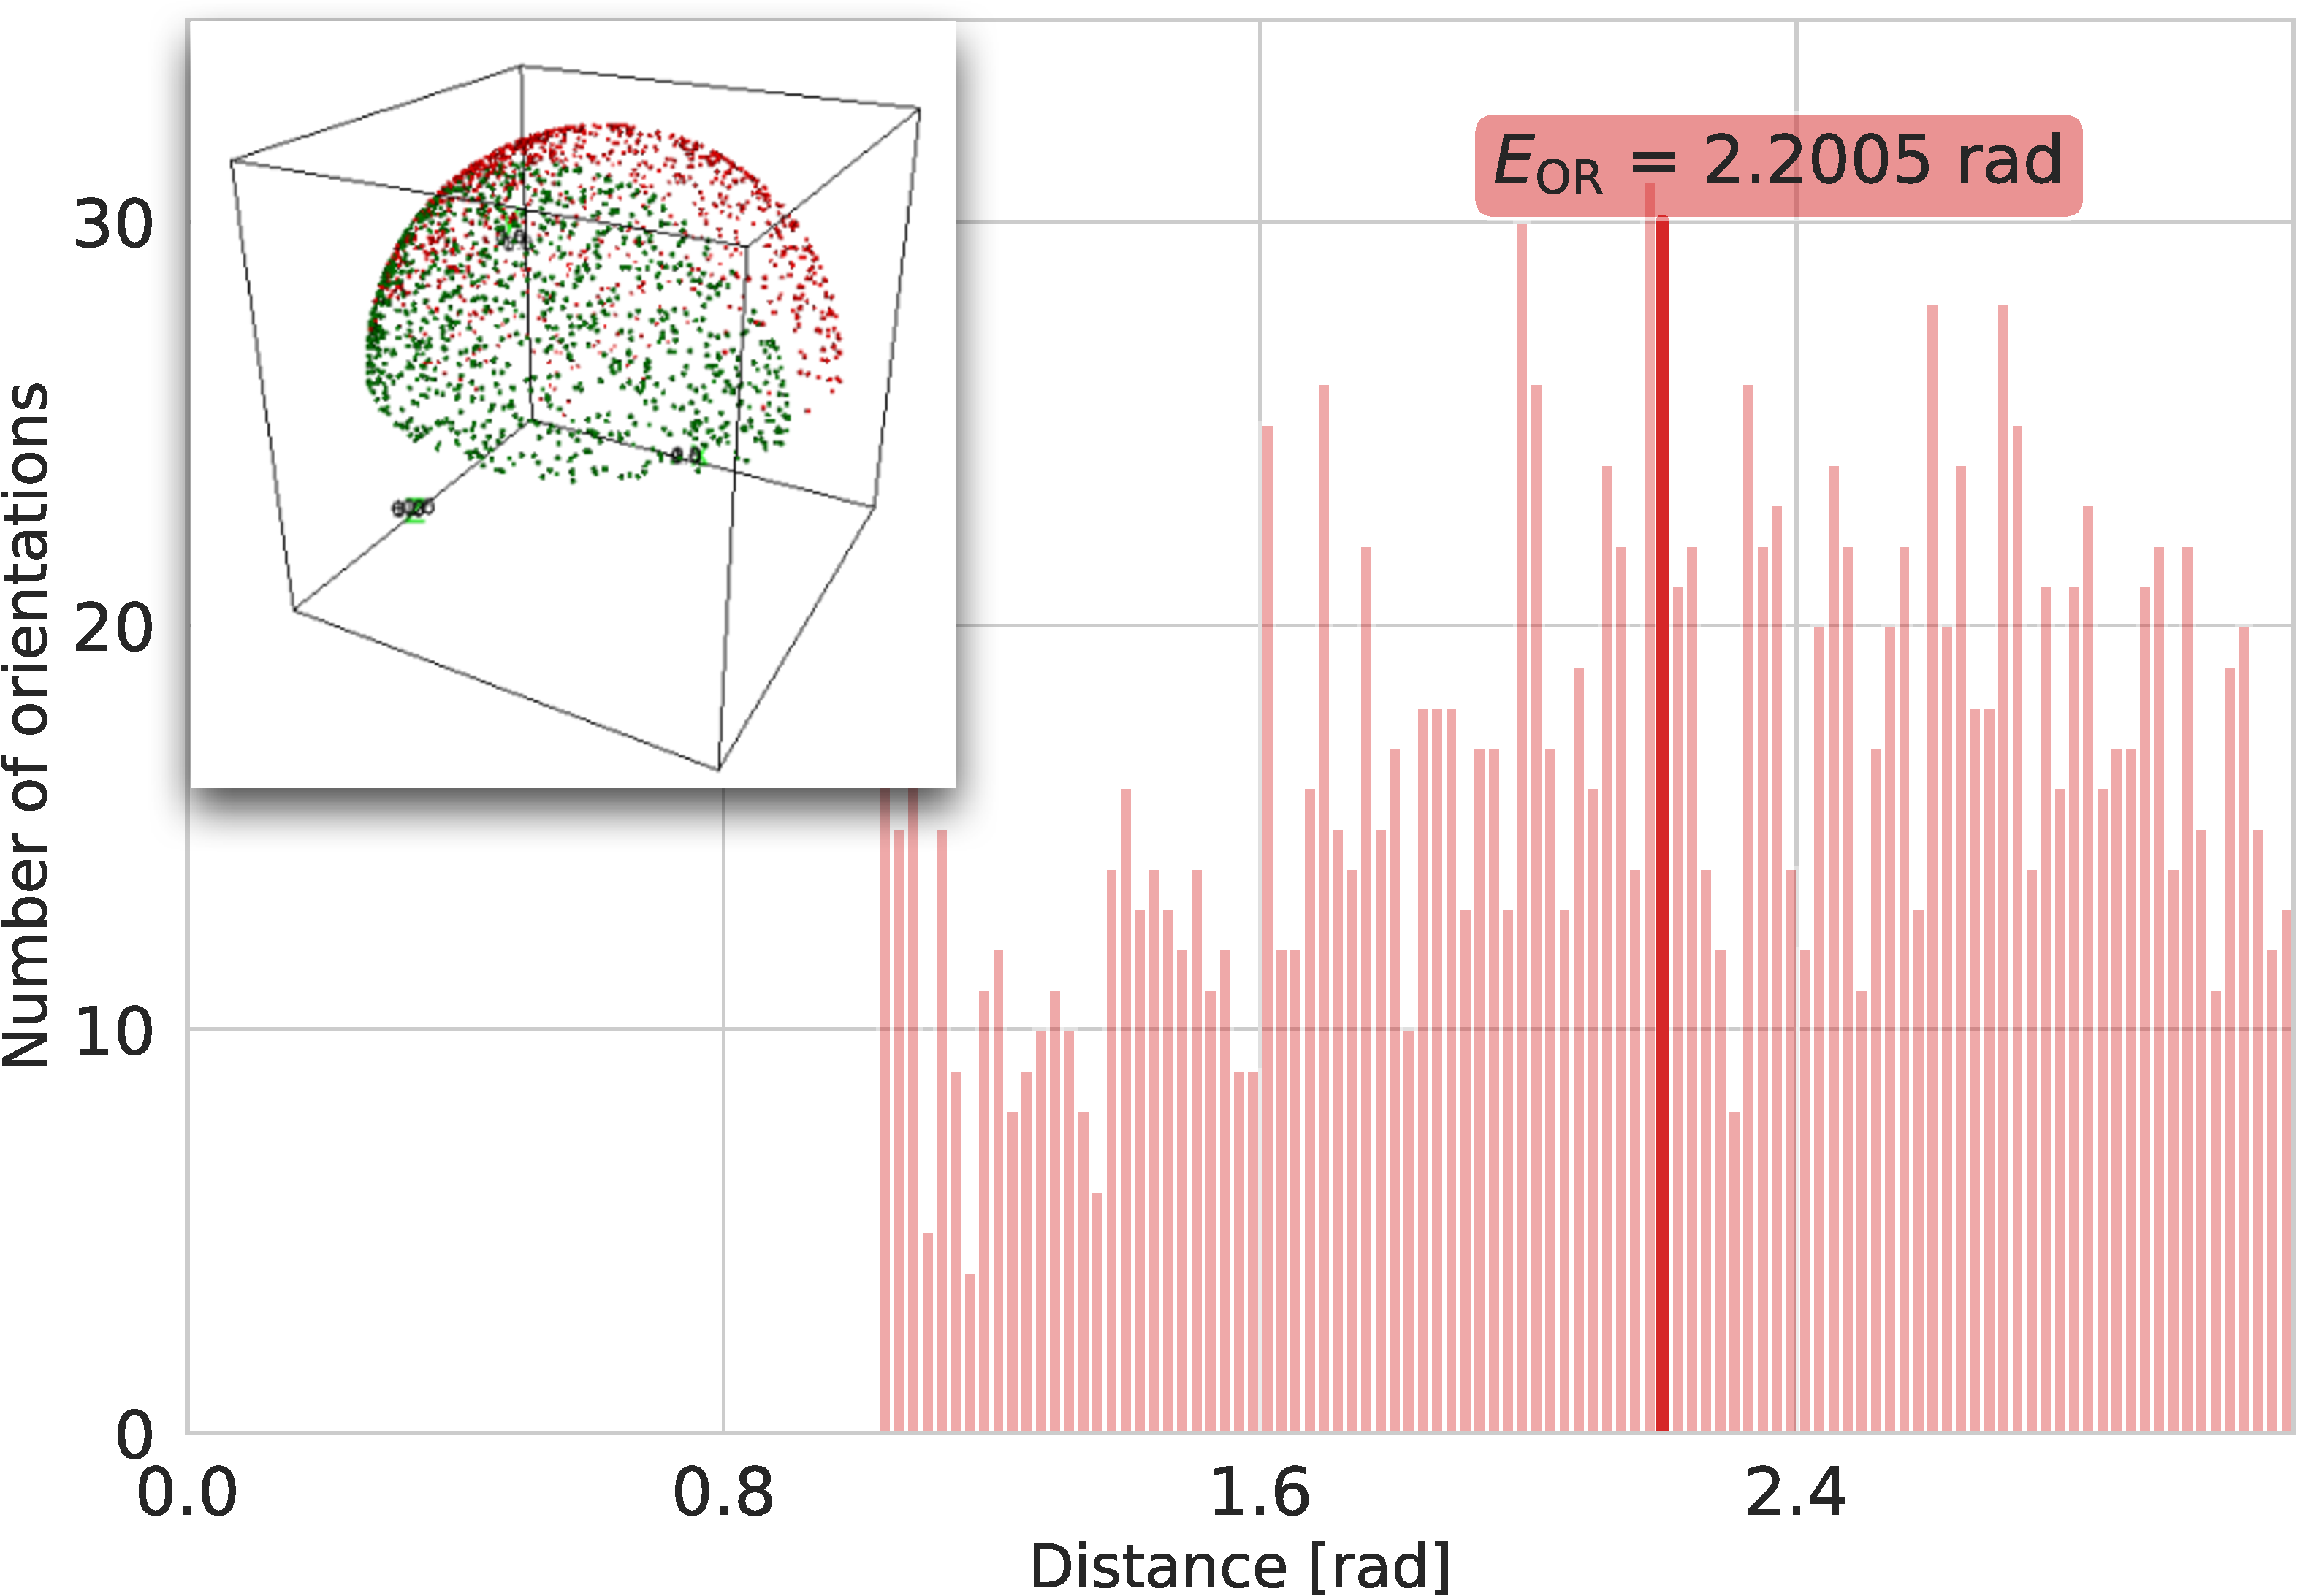
\includegraphics[height=3cm]{figures/BeforeAA.pdf}
            \caption{Orientations before alignment.}
        \end{subfigure}
        \hfill
        \begin{subfigure}[t]{0.46\linewidth}
            \centering
            % 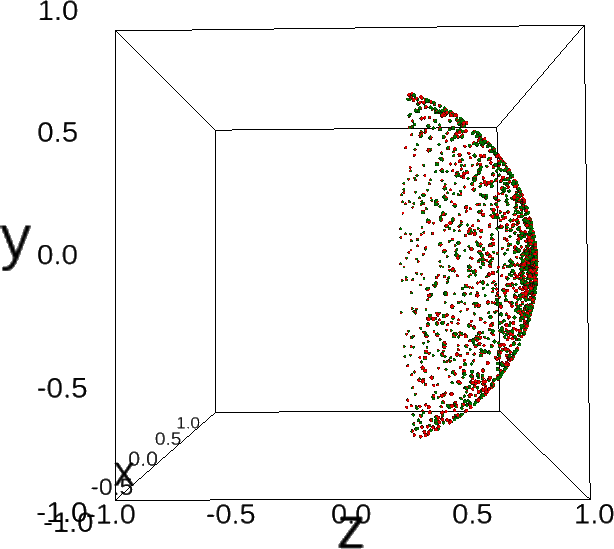
\includegraphics[height=3cm]{figures/coverage_alignment_after.png}
            %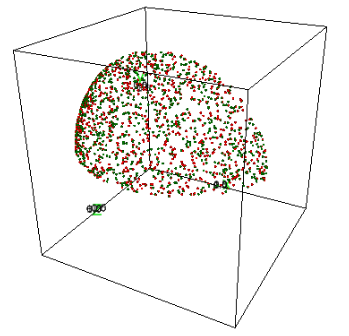
\includegraphics[height=3cm]{figures/after_aa.png}
            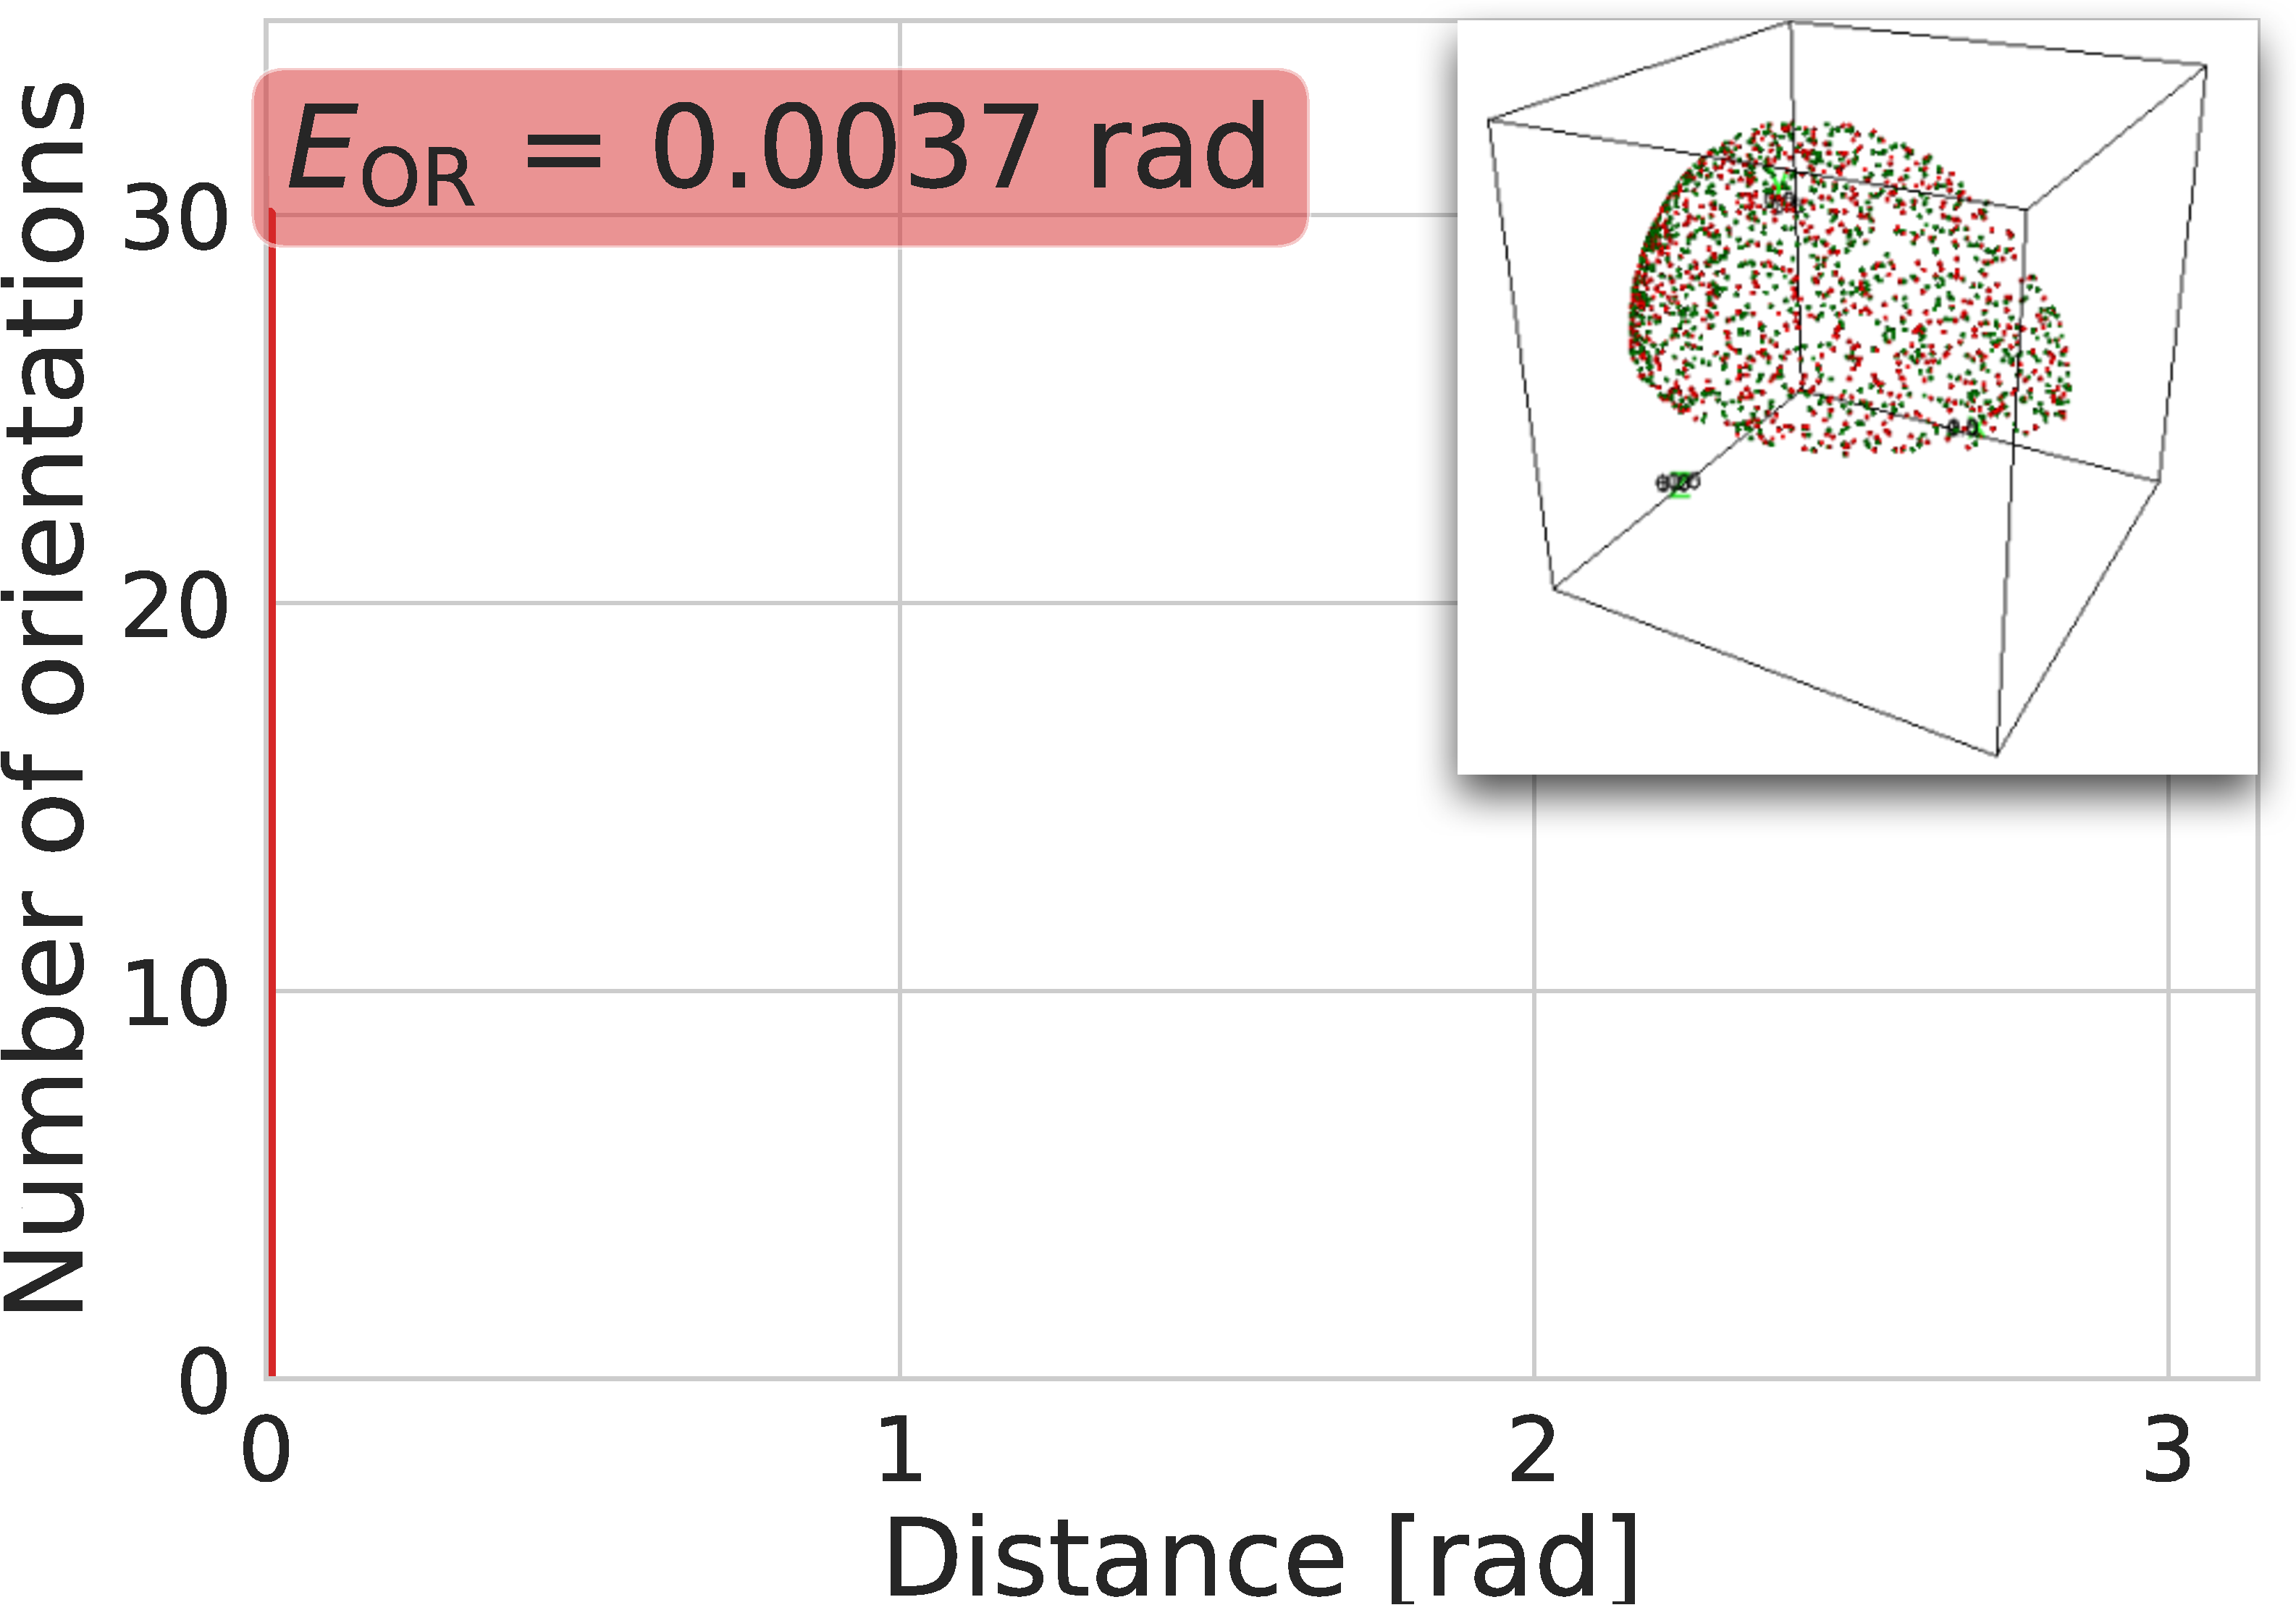
\includegraphics[height=3cm]{figures/AfterAA.pdf}
            \caption{Orientations after alignment.}
        \end{subfigure}
        \caption{%
            Example of perfect alignment~\eqnref{orientation-recovery-error} after a perfect orientation recovery~\eqnref{orientation-recovery}.
            The alignment error with corresponding directions $(\theta_2, \theta_1)$ before (a) and after (b) alignment.
            % and $\T$ as the optimum of \eqnref{orientation-recovery-error} on the right.
            %(b-c)~show the orientations projected on $\mathbb{S}^2 \subset \SO(3)$ before (b) and after (c) alignment.
            Green points are the true orientations $\{q_i\}$ and red points are the recovered orientations $\{\widehat{q_i}\}$.
            % The Figure (b) is exactly aligned which can be seen when zoomed. Due to plotting artifacts,
            While both colors are seen in (b), they are exactly superimposed.
            \todo{Would be nice to have the same ticks and labels for the x-axis and y-axis of both plots.}
        }\label{fig:5j0n-aa-loss-perfect-distances}
    %    \label{fig:angle-alignment-perfect}
    \end{minipage}
\end{figure}

\section{Euclidean distance between projections}\label{apx:results:distance-estimation}
% Orientation distance as, Estimating distances with

%\mdeff{Story: simplest baseline estimator, $d_{pe}$ somewhat estimates $d_q$, quickly plateaus (even in the simplest noiseless and centered case).
%Note the difference between symmetric and asymmetric proteins.}

\todo{Copy-edit.}

We evaluate $d_p(\p_i, \p_j) = \Vert \p_i - \p_j \Vert_2$ (\ie, the Euclidean distance) as a baseline distance estimator.
From $P = 5,000$ possible projection, we randomly select $5$ projections.
For each of these projections, we compute the Euclidean distance between aforementioned projection and all the others $d_p(\mathbf{p}_i,\mathbf{p}_j)=\lVert\mathbf{p}_i-\mathbf{p}_j\rVert_2$ and their corresponding orientation distance $d_q(q_i,q_j)$ through~\eqnref{distance:orientations}.
We then report the $(d_q,d_p)$ relationship for all pairs in \figref{euclidean-not-robust}, for both the \texttt{5j0n} (left) and \texttt{5a1a} (right).

Two principal observations can be made from this experiment.
First, as suspected, $d_p$ fails to be a consistent predictor of $d_q$, even in the simple imaging conditions considered here (no noise, no shift, no PSF).
In particular, the larger the quaternion distance $d_q$, the poorer the predictive ability of $d_p$ (the plot plateaus).
The other interesting observation is that the trend of $(d_q,d_p)$ plot of the \texttt{5a1a} appears to take symmetric shape of letter \texttt{M} which can be explained with the fact that this protein has intrinsic dihedral (D2) symmetry~\cite{noauthor_d2sym_nodate,noauthor_5a1asym_nodate}.
\mdeff{Check these refs. Other ones are used in main text?}

\begin{figure}[ht!]
    \begin{minipage}[t]{0.52\linewidth}
        \begin{subfigure}[t]{0.48\textwidth}
            \centering
            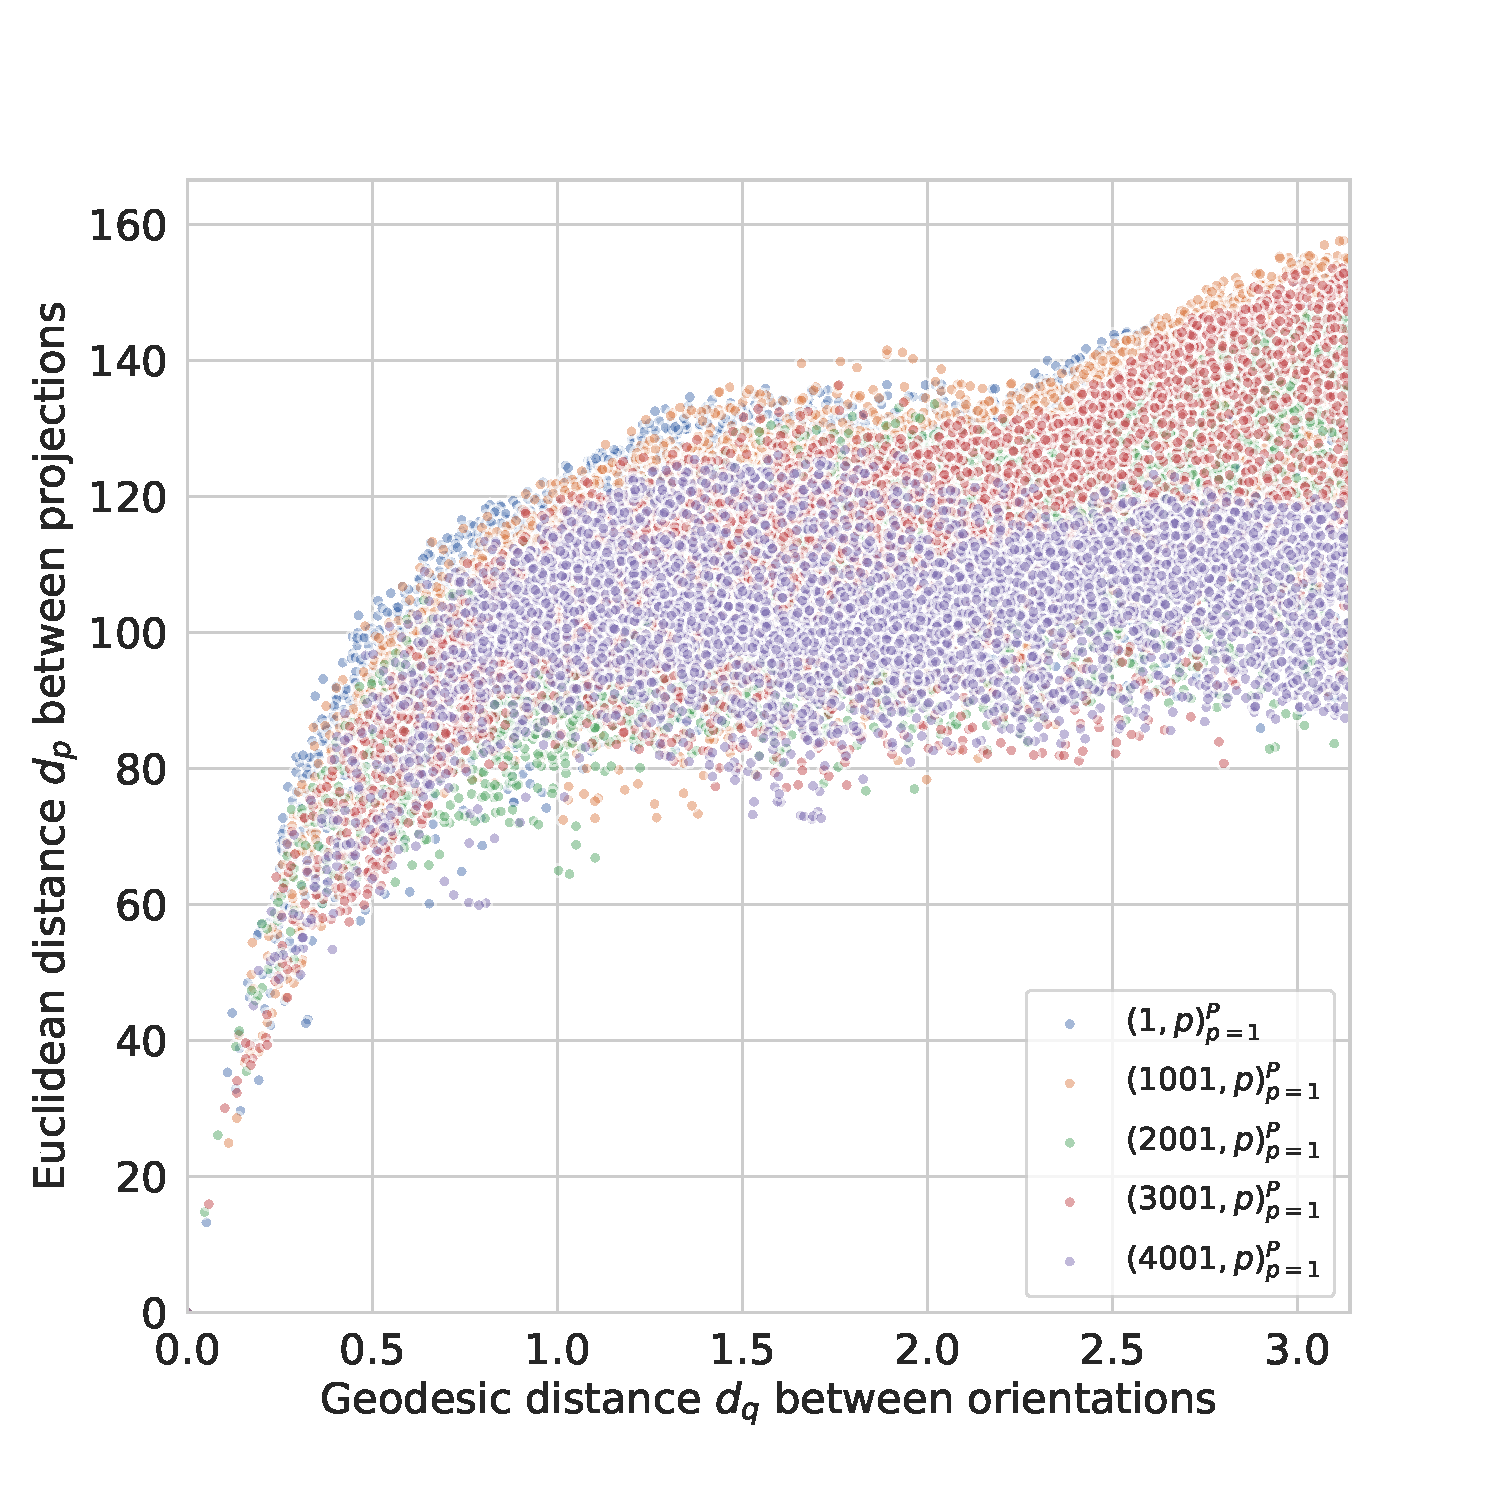
\includegraphics[height=4cm]{figures/eucl_notrobust_5j0n}
            \caption{\texttt{5j0n}}
        \end{subfigure}
        \hfill
        \begin{subfigure}[t]{0.48\textwidth}
            \centering
            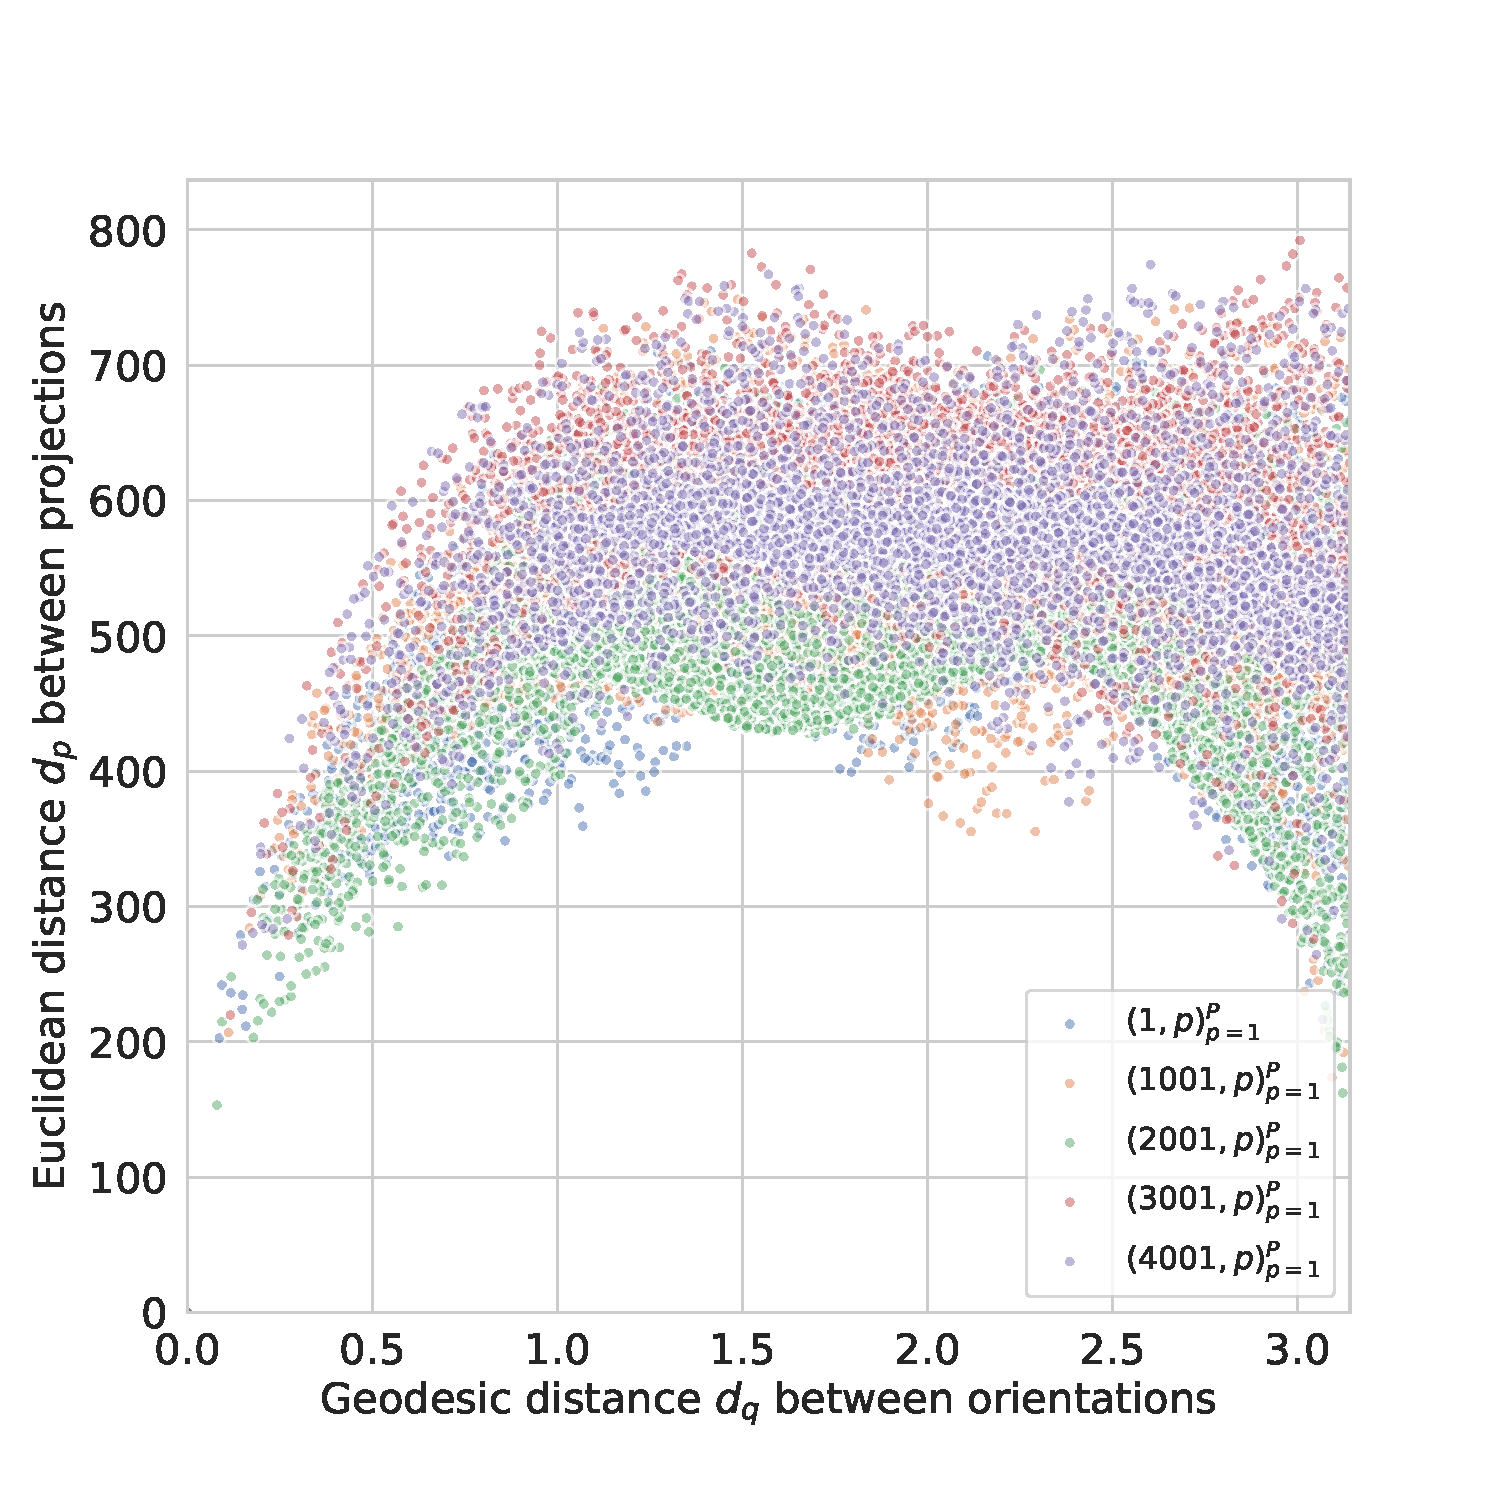
\includegraphics[height=4cm]{figures/eucl_notrobust_5a1a}
            \caption{\texttt{5a1a}}\label{fig:euclidean-not-robust:5a1a}
        \end{subfigure}
        \caption{%
            The Euclidean distance between two projections $d_p(\p_i, \p_j) = \Vert \p_i - \p_j \Vert_2$ versus their actual relative orientation $d_q(q_i, q_j)$ with the half-sphere direction coverage.
            Each color represent the distances between one fixed projection and the other $P-1$ projections.
    %        The color corresponds to projection pairs that share one projection, \ie, distance between one projection with all other projections.
            While there is some correlation, especially at small distances, the Euclidean distance is a poor estimator.
            Because \texttt{5a1a} has D2 symmetries, two projections might be identical while not having been acquired from the same orientation.
            \mdeff{Is there a reason (other than historical) for those dPdQ plots to be different (w.r.t.\ how distances are sampled) from the ones in \figref{distance-learning:dpdq} and \figref{geo-eucl-mlp}?}
        }\label{fig:euclidean-not-robust}
    \end{minipage}
    \hfill
    \begin{minipage}[t]{0.43\linewidth}
        \centering
        % 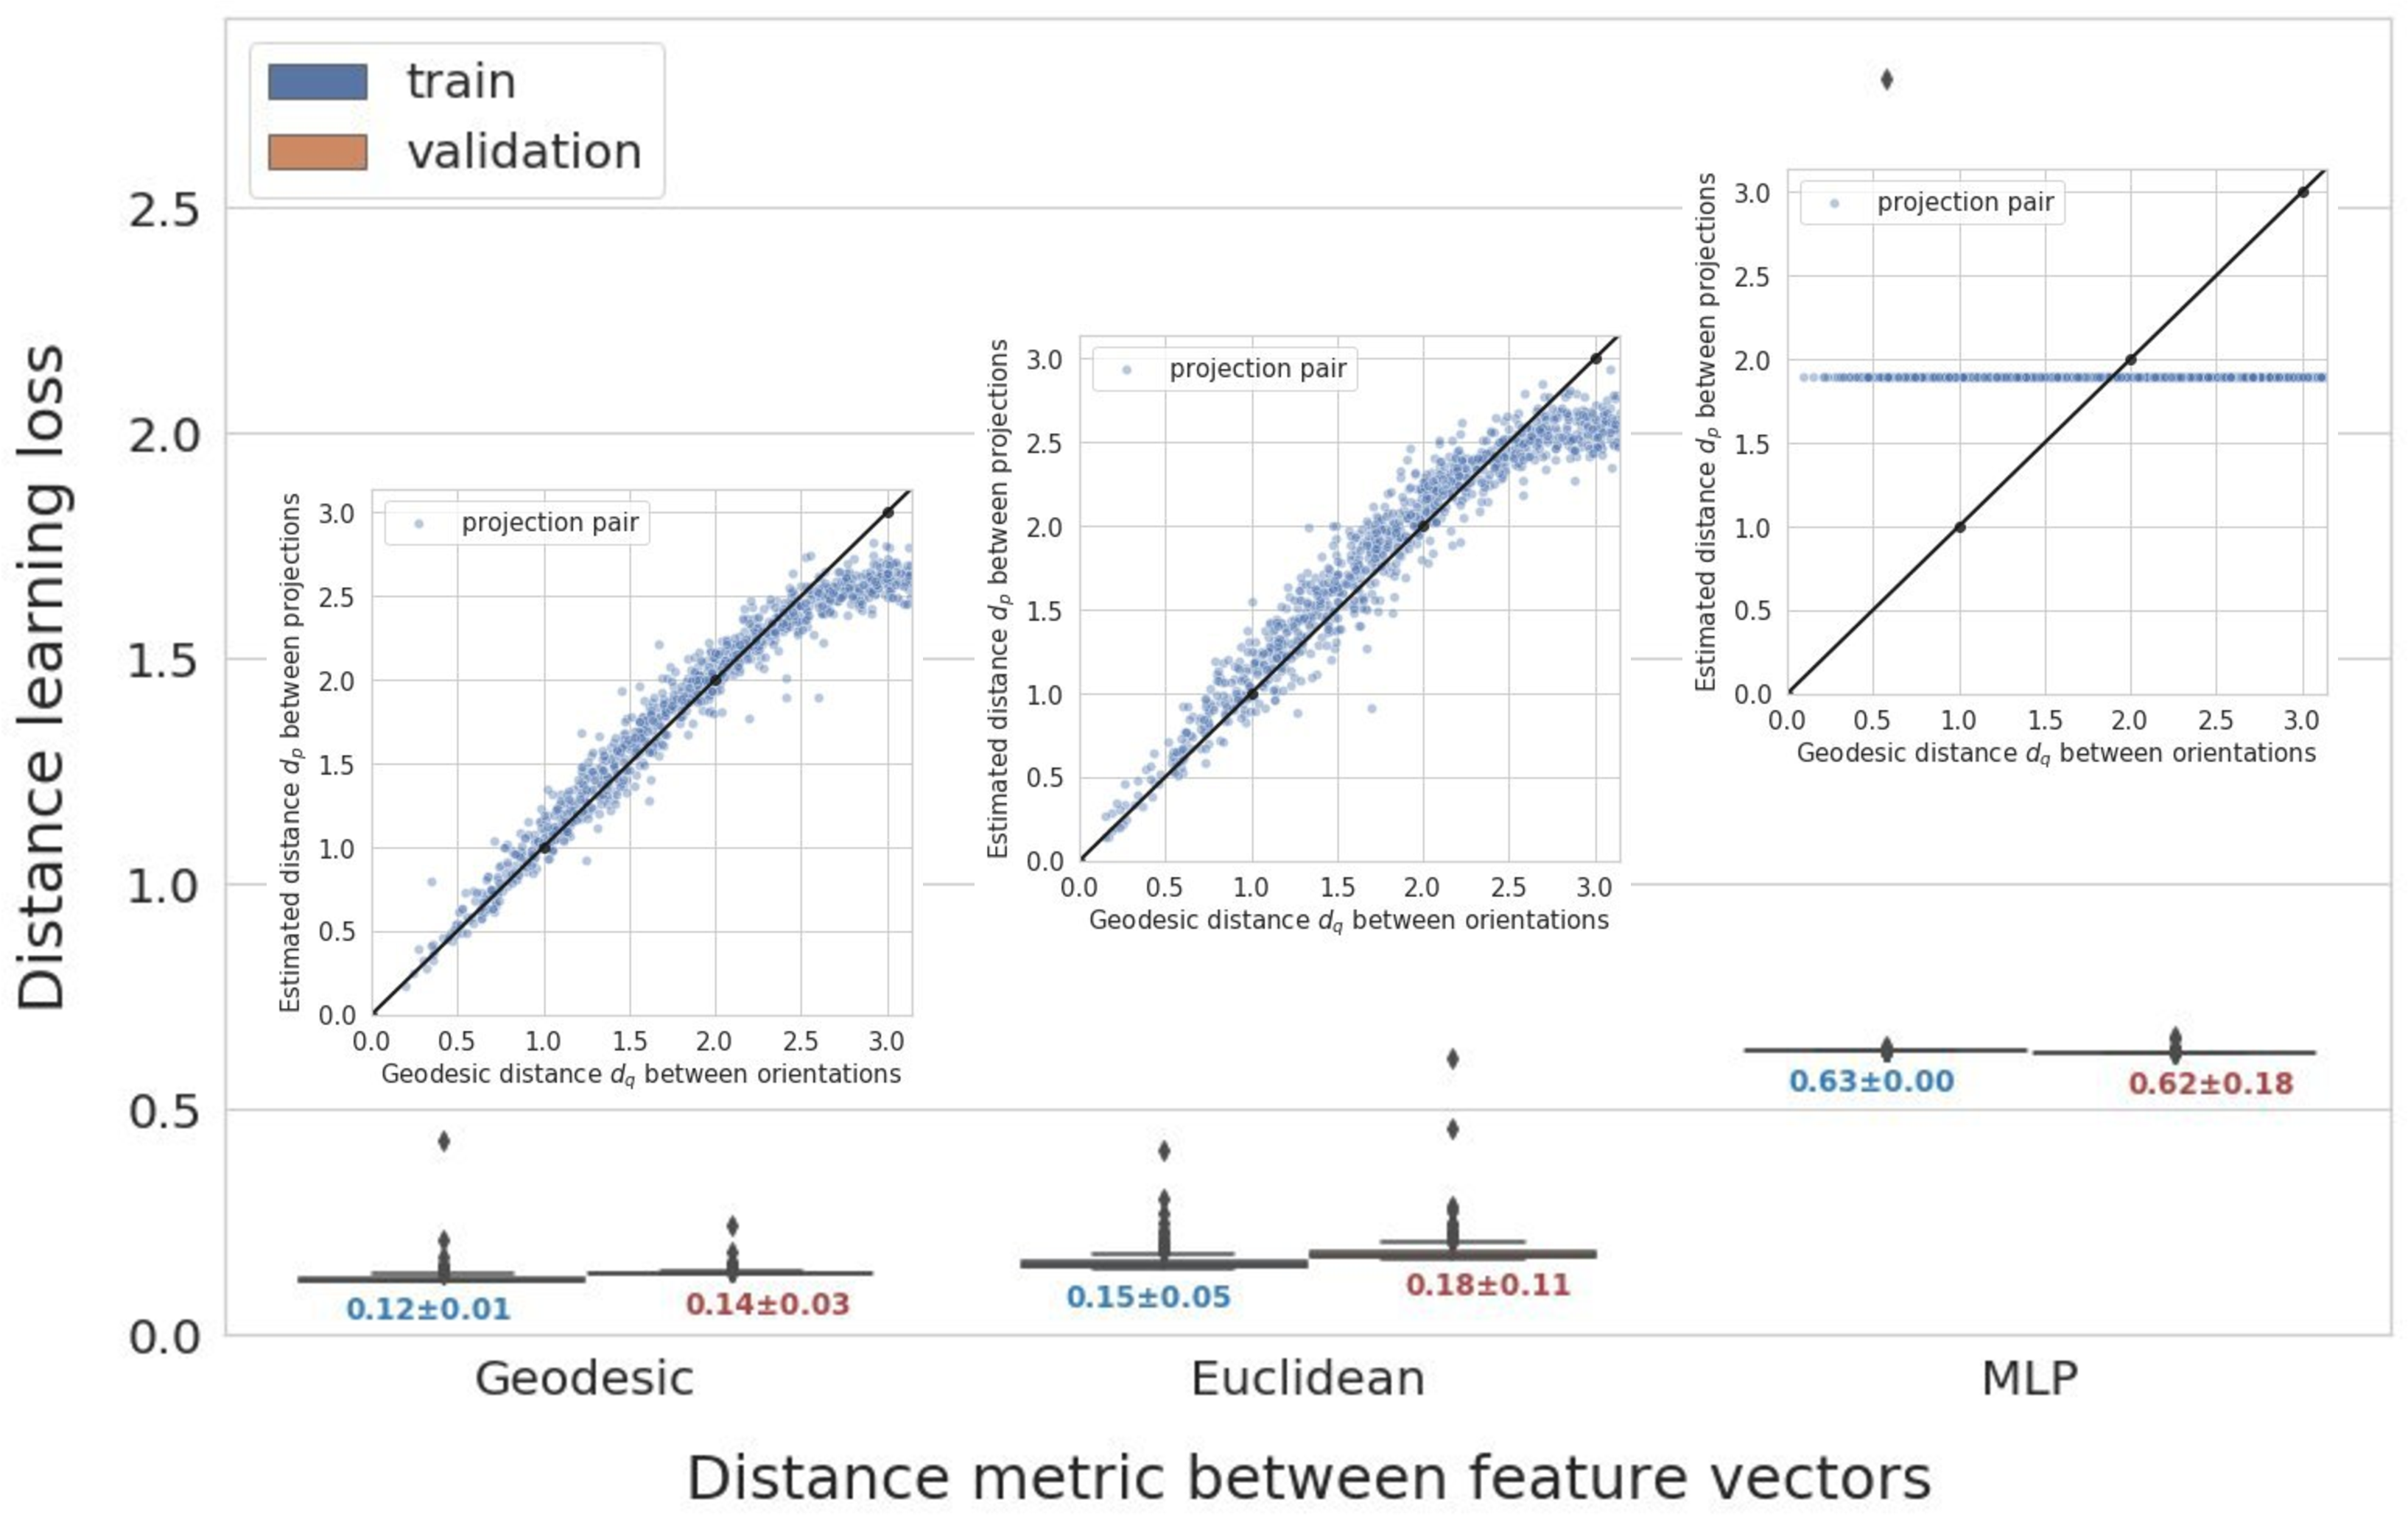
\includegraphics[height=4cm]{figures/geo_eucl_mlp_distance_metric.pdf}
        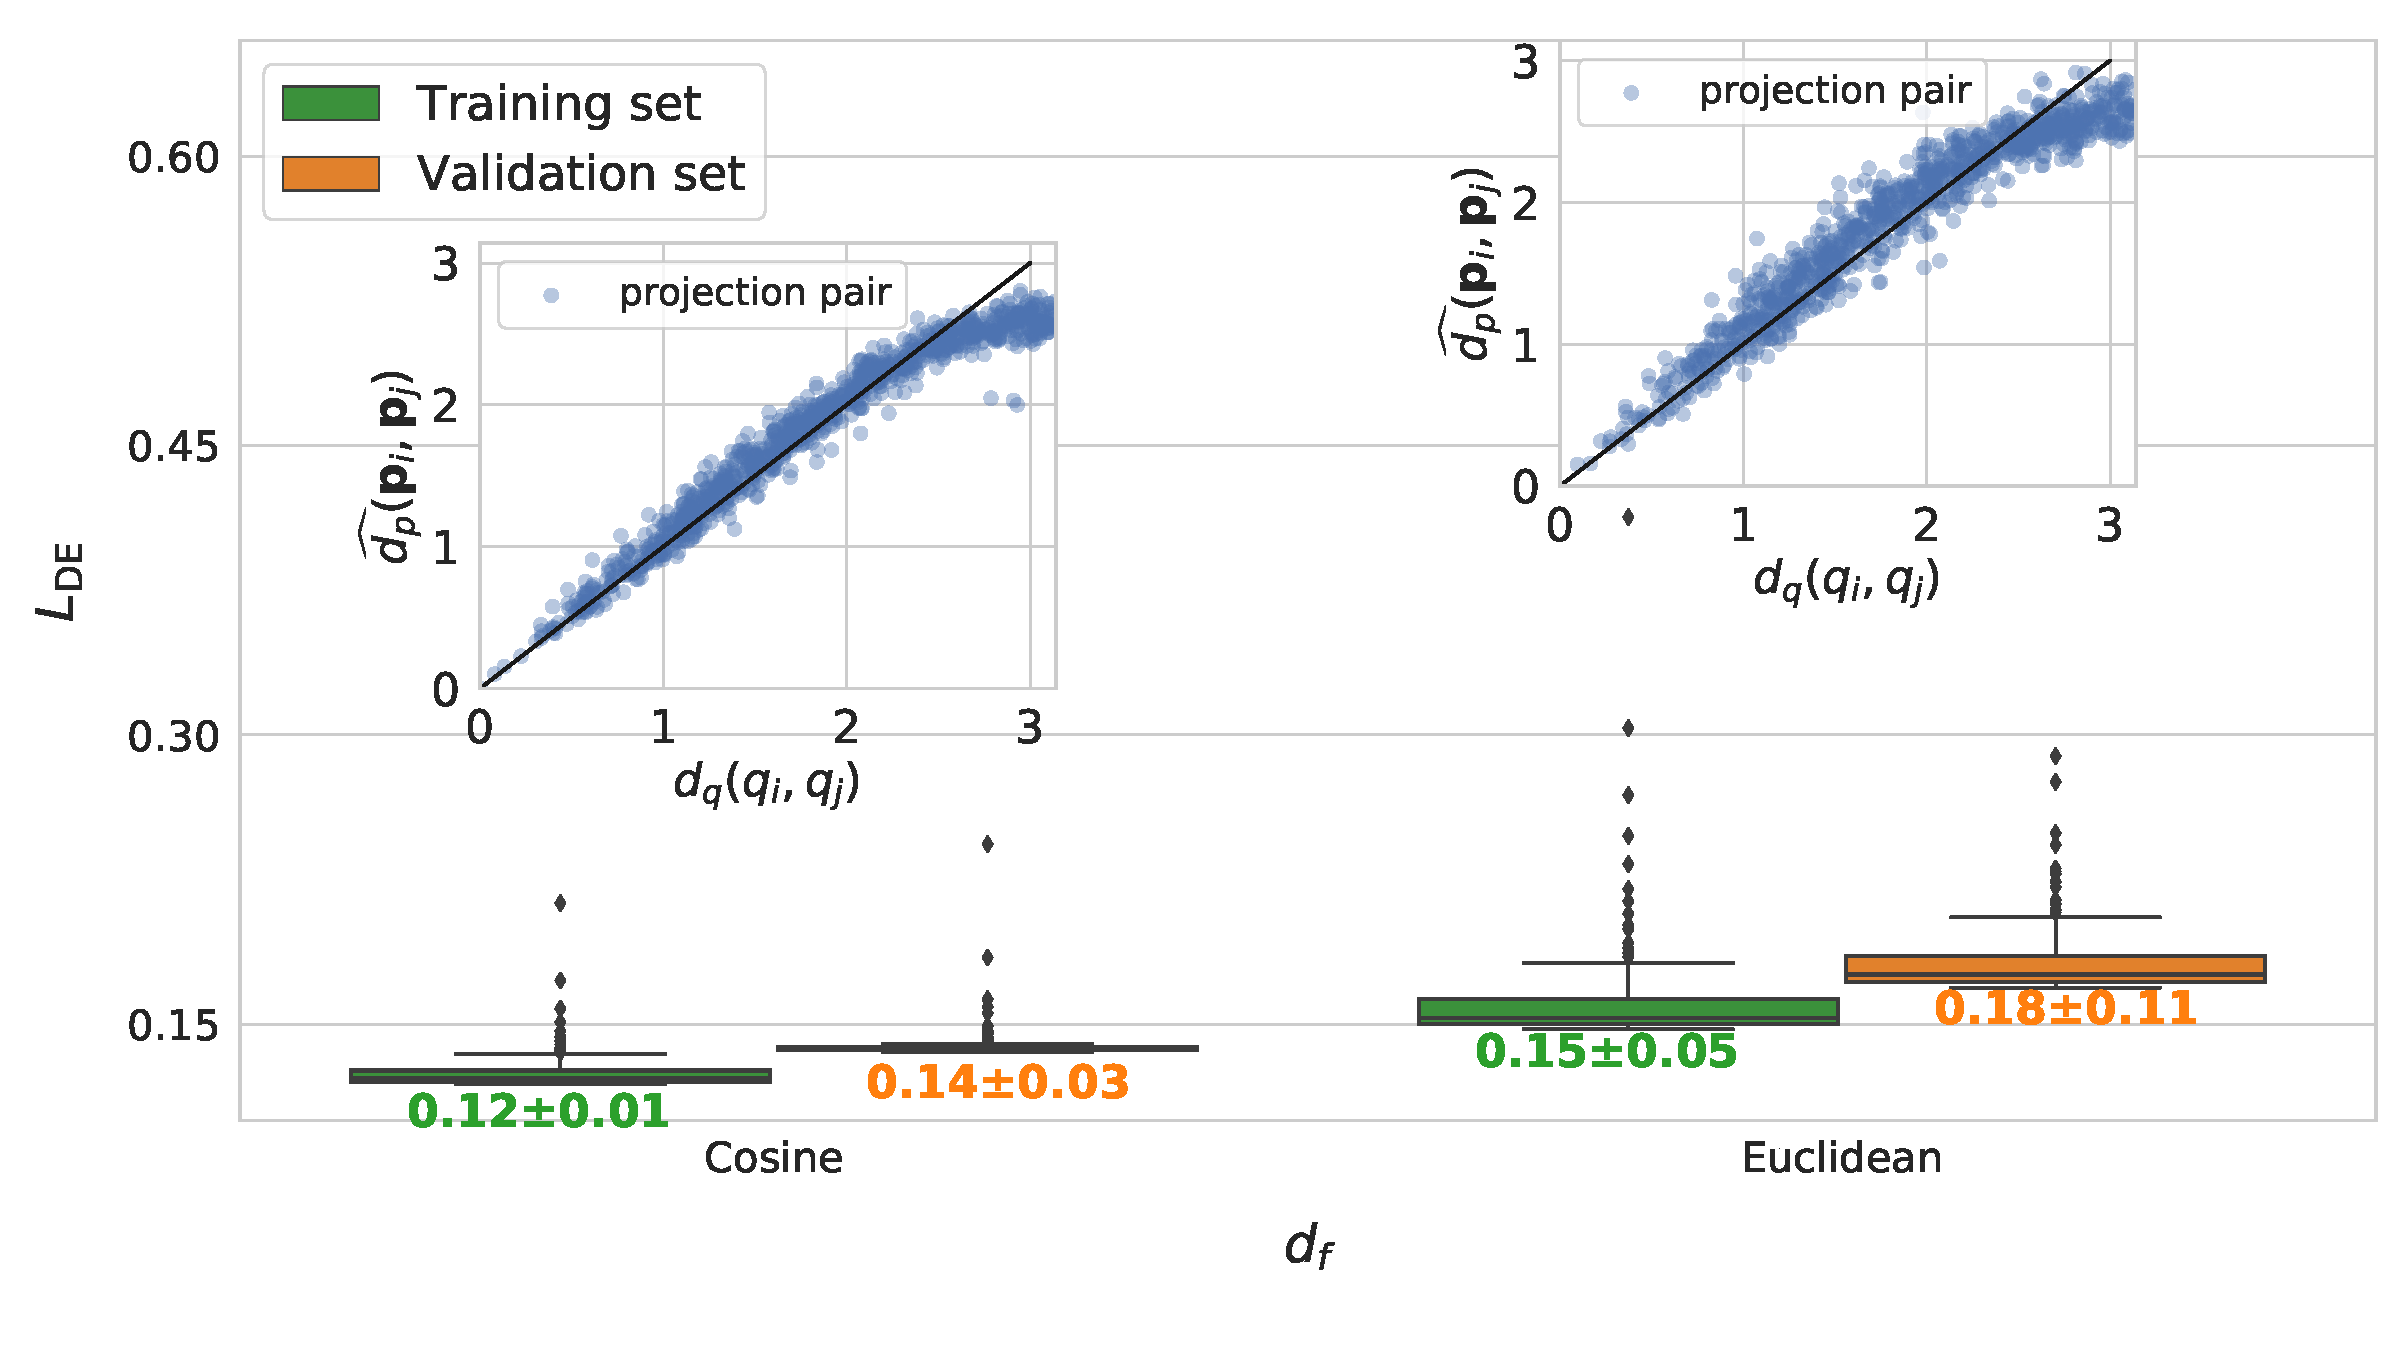
\includegraphics[height=4cm]{figures/dPdQ_feat_distances.pdf}
        \caption{%
            Performance of distance learning w.r.t.\ the choice of feature distance function $d_f$.
            The box plots show the distance learning loss $L_\text{DE}$ \eqnref{distance-learning} on the training (blue) and validation (red) sets.
            The inserted plots show the relationship between $d_q(q_i, q_j)$ and $d_p(\p_i, \p_j) = d_f(\mathcal{G}_w(\p_i), \mathcal{G}_w(\p_j))$.
            %\todo{Consistency: train -> training set, validation -> validation set, and Geodesic -> Cosine. Add $L_\text{DE}$ to the y-axis label. Larger text.}
            %\todo{Remove the MLP results. It didn't work at all. Make the difference between Euclidean and Cosine easier to see.}
        }\label{fig:geo-eucl-mlp}
    \end{minipage}
\end{figure}

\section{Choice of feature distance}\label{apx:feature-distance}

%\mdeff{Story: $d_f = d_q$ better than Euclidean and MLP $d_f$. }

There are multiple options for a distance function $d_f$ between two features $\mathbf{f}_i = \mathcal{G}_w(\p_i) \in \R^{n_f}$. We compared the performance of three different distances:

\begin{itemize}
    \item the Euclidean distance, \ie, $d_f(\mathbf{f}_i, \mathbf{f}_j) = \| \mathbf{f}_i - \mathbf{f}_j \|_2$
    \item the cosine distance, \ie,
$ d_f(\mathbf{f}_i,\mathbf{f}_j) = 2 \arccos \left( \frac{\langle \mathbf{f}_i, \mathbf{f}_j \rangle}{\lVert \mathbf{f}_i \rVert \lVert \mathbf{f}_j \rVert} \right)$
\todo{No absolute value. So not as in \eqnref{distance:orientations}.}
    \item the parametrization of $d_f$ as a multi-layer perceptron (MLP) whose parameters are learned.
\end{itemize}

The MLP we tested was made of six layers with $1024, 512, 512, 256, 256, 1$ units, all of which use the SeLU activation function. The features $\mathbf{f}_i$ and $\mathbf{f}_j$ were stacked as an array of size $2n_f$ before being fed to the MLP\@. Note that, while a MLP can approximate any function, there is no guarantee that the learned function will satisfy the axioms of a proper distance function (\ie, the identity of indiscernibles, symmetry, and triangle inequality). \lau{Say that we were not able to train.}

\figref{geo-eucl-mlp} compares the use of the first two distances. The Euclidean distance yields better results, but the cosine distance is ultimately the best performer of all: $L_\text{DE}$ is the lowest, which makes $d_p$ a better estimator of $d_q$.
% the projection pairs deviate the least from the identity
This superiority of the cosine distance is likely due to its capacity to model the elliptic geometry of $\SO(3)$, a feat the Euclidean distance does not achieve, the Euclidean space being neither periodic nor curved.
%The $\SO(3)$ is non-linear and it can be explained with the fact that Euclidean distance of two quaternions can be small, despite the rotation being large~\cite{huynh_metrics_2009,DBLP:journals/corr/abs-1805-01026}.

\section{Estimating distances on unseen proteins}\label{apx:unseen-proteins}
%\section{Non-determinism of the Orientation Recovery}\label{apx:non-determinism}

As the SiameseNN will ultimately be trained on known proteins and used to estimate distances on unknown proteins to be imaged,
%we also desire our learned distance function to generalize/transfer across density maps $\x$.
we also desire our learned distance function to generalize to unseen proteins.
The distance function $\widehat{d_p}$ must abstract the protein---in the same way it must abstract shifts, noise, or PSFs to generalize to unseen projections.
We attempted to recover the orientations of noiseless projections from \texttt{5j0n} while we had trained the SiameseNN on $4,000$ noiseless projections from four other proteins (\texttt{5nvu}~\cite{ZHANG20171303}, \texttt{5nvs}~\cite{ZHANG20171303}, \texttt{6mem}~\cite{iwai2018unique}, \texttt{6o1o}~\cite{liu2019target}, which have the same type of symmetry as \texttt{5j0n}).
%In this experiment, we generated $1,000$ projections per protein.
%\todo{should be the same ``kind'' of refs as the ones used in 3.1 for \texttt{5j0n} and \texttt{5a1a}}
%Four proteins were used in the training and validation set to ensure the robustness to the unseen protein \texttt{5j0n} used in the testing set.
%The number of projections in every set is the same as in \tabref{dataset}.
We obtained a recovery loss of \todo{$L_\text{OR} = 0.0352$},
to be compared with \todo{$L_\text{OR} \approx 0.11$} when the SiameseNN was trained on \texttt{5j0n} alone.
While performance is somewhat degraded, we conclude that it is possible to train and use a distance function on different proteins.

\todo{Distance learning and orientation recovery worked well, but alignment didn't.}
\mdeff{Why is dPdQ so bad? Seems contradictory to a low $L_\text{DE}$ and $L_\text{OR}$. Maybe that's why alignment didn't work? But then I don't get why $L_\text{DE}$ and $L_\text{OR}$ are so low\ldots.}

\mdeff{Could we also have $E_\text{OR}$? It's easier to understand and compare.}
\banjac{I fully agree, however, I already mentioned that I wasn't able to align the orientations even though the $L_\text{OR}$ was very good. Looking at the estimation and GT in rotation space, it is visible we have some kind of transformation between these two (transformation similar to one we found the flip is causing, but it is not the flip).}
\mdeff{Could we show the ground-truth and estimated orientations in \figref{robustness-to-unseen-pipeline}?}

\begin{figure}[ht!]
    \centering
    \begin{subfigure}[b]{0.35\linewidth}
        \centering
        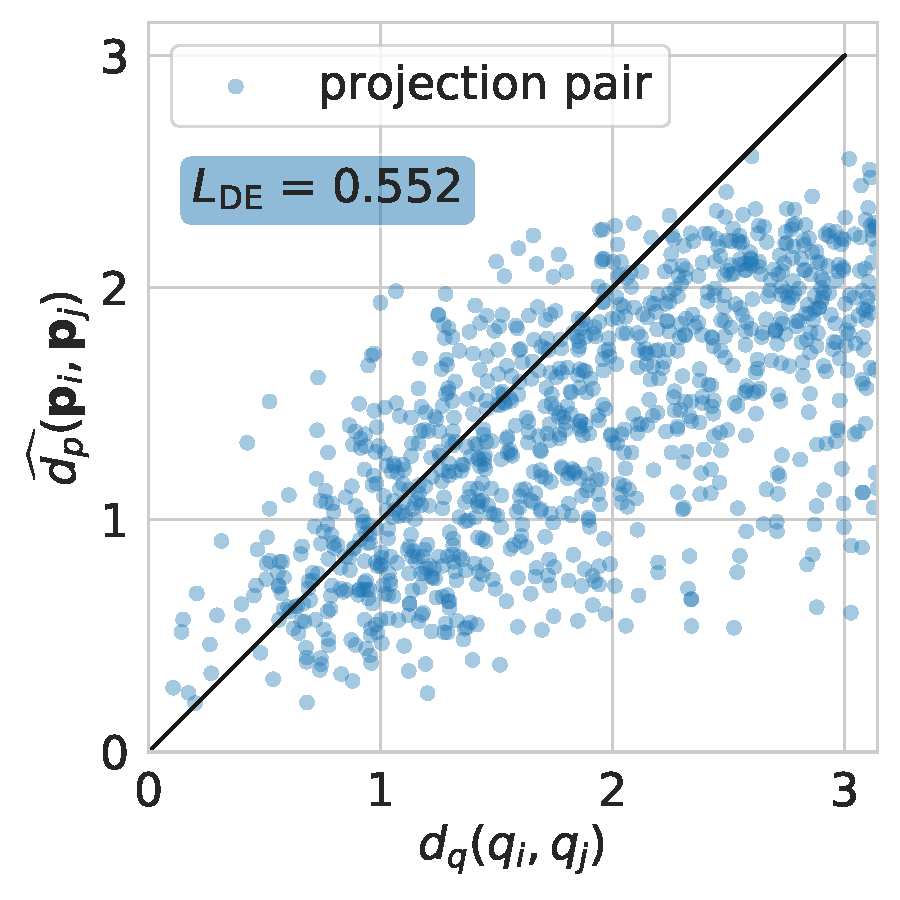
\includegraphics[height=11em]{figures/dPdQ_5j0n_robustness_to_unseen.pdf}
        \caption{Relationship between $\widehat{d_p}$ and $d_q$ on $1,000$ pairs sampled from the \texttt{5j0n}.}
    \end{subfigure}
    \hfill
    \begin{subfigure}[b]{0.55\linewidth}
        \centering
        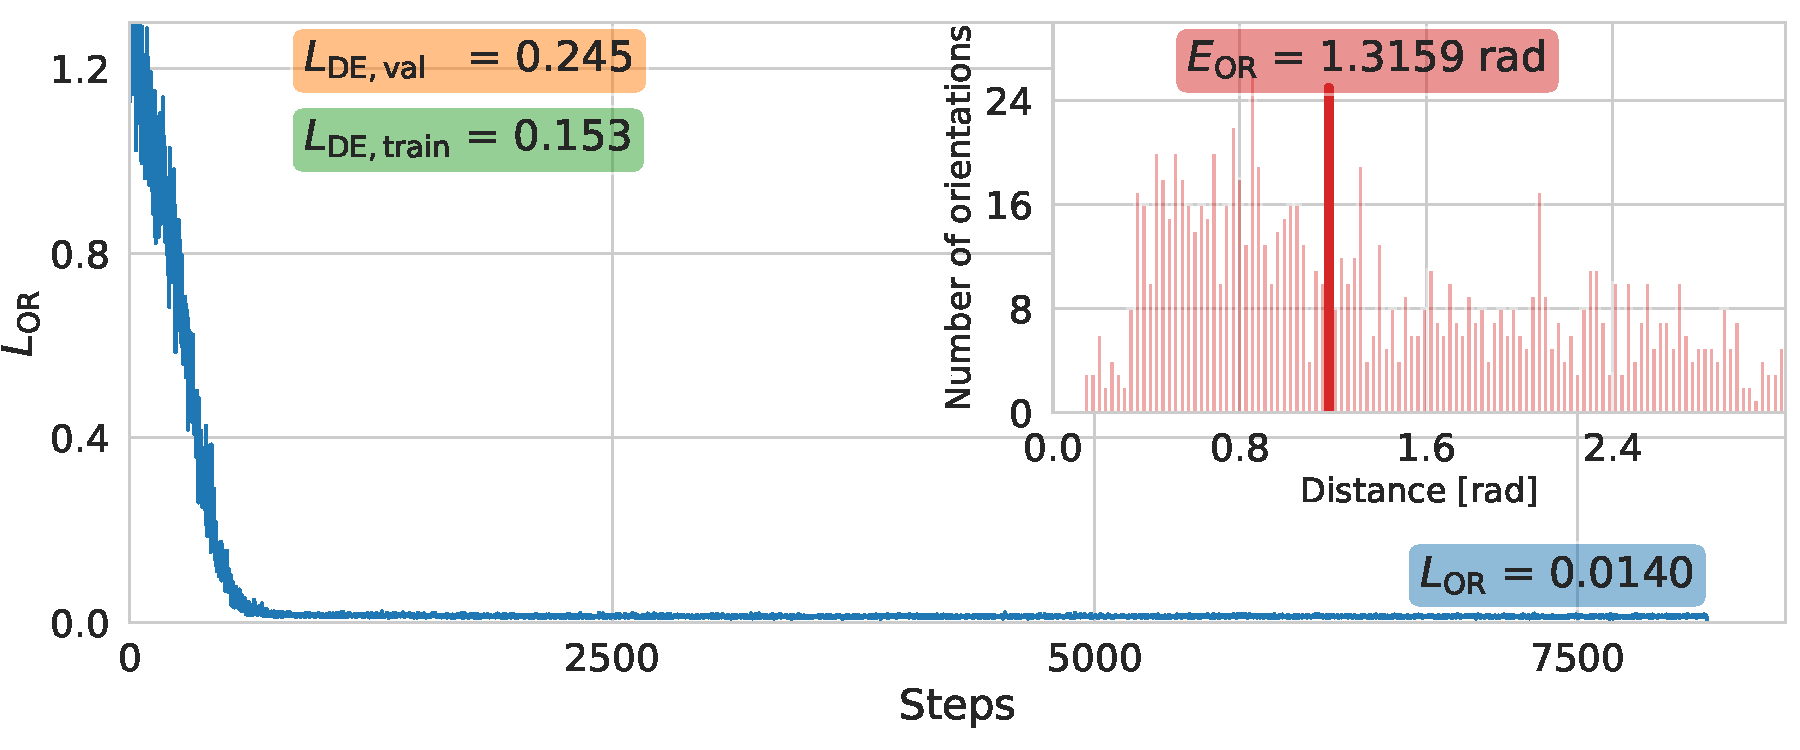
\includegraphics[height=11em]{figures/5j0n_ar_aa_robustness_to_unseen.pdf}
        \caption{Recovered $\{ \widehat{q_i} \}$ from noiseless \texttt{5j0n} projections $\{ \p_i \}$ from protein unseen from distance estimation algorithm.}
    \end{subfigure}
    \caption{%
        Robustness to unseen protein \texttt{5j0n} pipeline results.
    }\label{fig:robustness-to-unseen-pipeline}
\end{figure}

\clearpage
\section{SiameseNN architecture}\label{apx:siamese-architecture}

\begin{figure}[ht!]
    \centering
    \begin{subfigure}[t]{0.5\linewidth}
        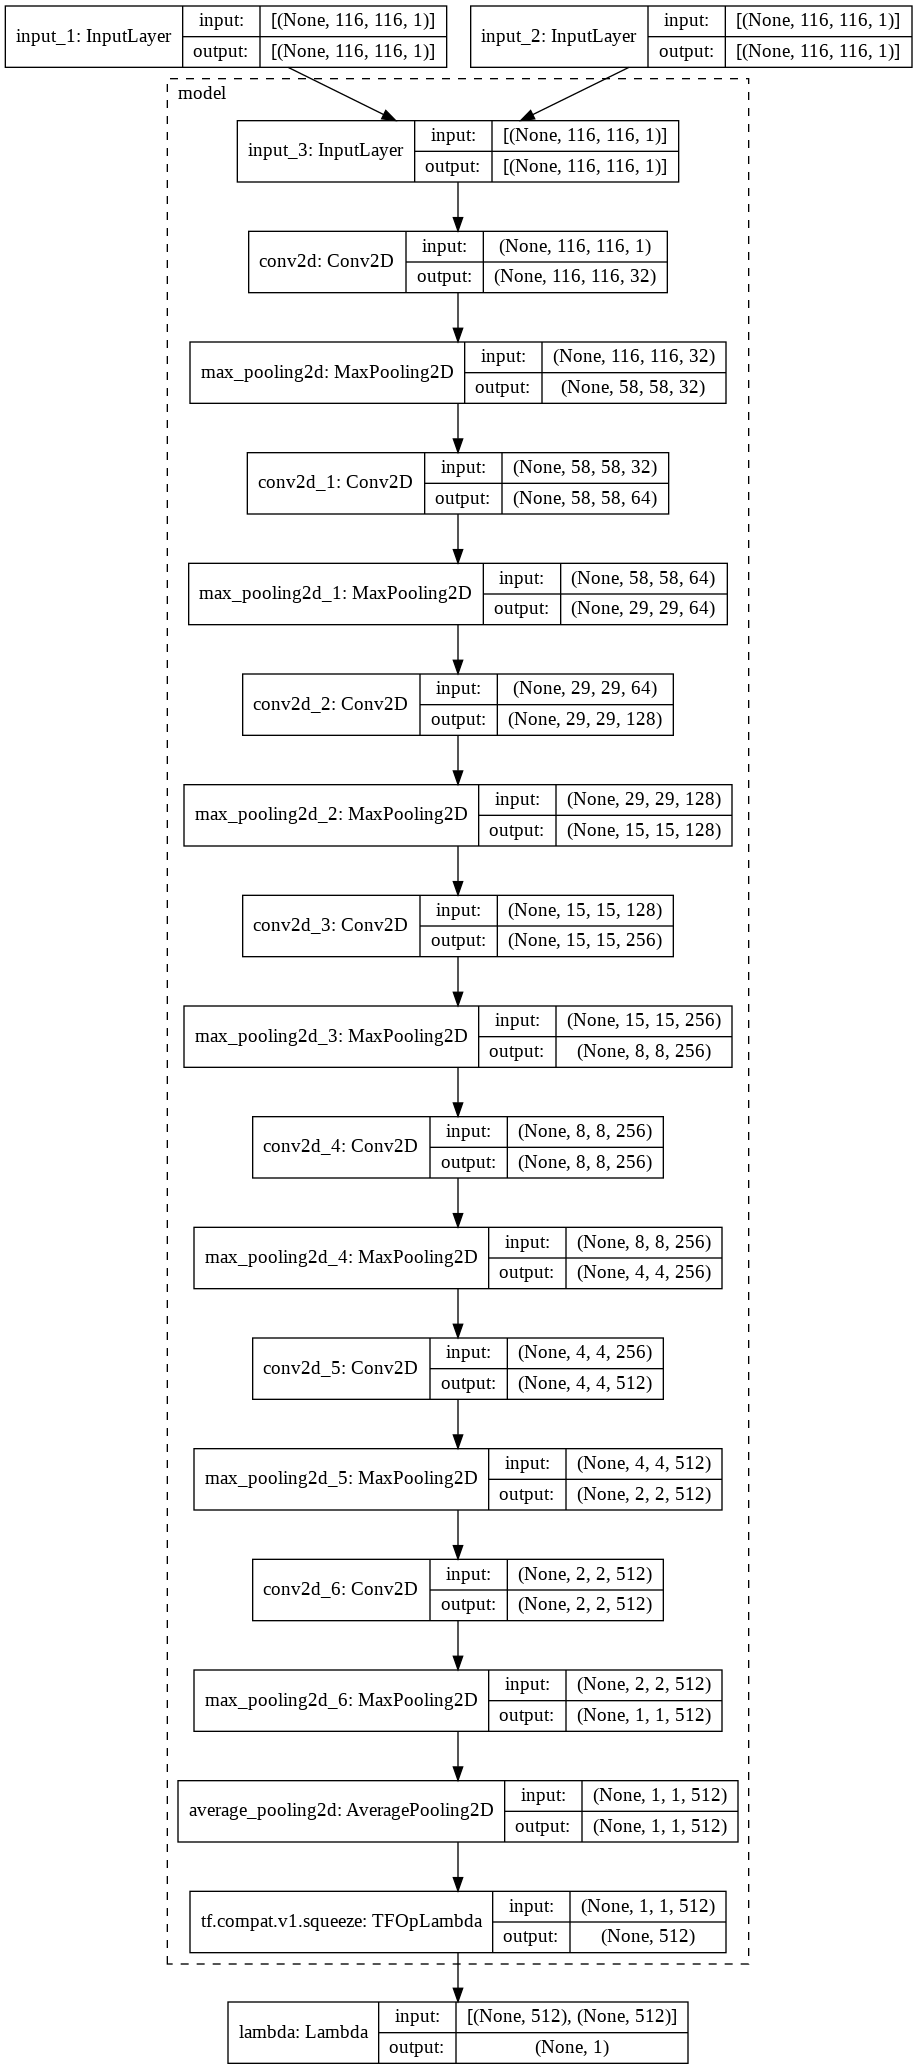
\includegraphics[width=\linewidth]{figures/model_plot_256d.png}
    \end{subfigure}
    \caption{%
        Distance estimation network architecture.
        We have two input images of dimensions $116 \times 116$.
        Each one goes to its CNN (part where we share the weights, selected with a dashed line).
        The output is a scalar value representing the distance between these two images.
        Last layer converts feature vector to a higher-dimensional vector of size $n_f=256$. This architecture of network was used throughout all experiments. The last layer was different for $n_f=4$.
        %\mdeff{Those are two similar to warrant two figures. We can just say that the last layer is  different for $n_f=4$.}
    }\label{fig:de-architecture}
\end{figure}
